\documentclass[12pt,a4paper]{article} 

\usepackage[utf8]{inputenc}
\usepackage{amsmath}
\usepackage{amsfonts}
\usepackage{amssymb}
\usepackage{graphicx}
\usepackage{booktabs}
\usepackage{multirow}

\usepackage[english]{babel}
\usepackage[export]{adjustbox}
\usepackage{enumerate}

\usepackage[left=3.5cm,right=2.5cm,top=2.5cm,bottom=2.5cm]{geometry}

\usepackage{lineno}
\usepackage{tikz}
\usetikzlibrary{calc}


\begin{document}

	\begin{titlepage}



	\begin{tikzpicture}	[overlay, remember 					picture] \draw[line width= 1.3pt] ($(current 			page.north west)+(0.5in, -0.5in)$) rectangle ($			(current page.south east)+(-0.5in,0.5in)$);
	
	\end{tikzpicture}
	
	\begin{center}
		\begin{LARGE}			\bf{A Report on Field 			Trip to Barapukuria Coal Mine and Maddhapara 			Granite Mine\\}
		\end{LARGE}
		\vspace{10pt}
		\bf{Submission Date: \today}\\
		\vspace{30pt}
		Course title: Field Work(Mine Drainage and 				Dewatering System)\\
		Course Code: PME 434\\
		\vspace{30pt}
		
		\textit{Submitted by}\\
		\textbf{Tanveer Alam Munshi} \\
		\textbf{Reg No.: 2014336027}\\
		\textbf{Session: 2014-15}\\

		\vspace{20pt}
		
\includegraphics[width=0.45\textwidth]{logo.png}		
		\vspace{20pt}
		
		\textit{Under the kind guidance of}\\
		\vspace{10pt}
		\textbf{Mr Mahmudul Hasan}\\
		\textit{\textbf{Lecturer, Dept. of PME}}\\
		\vspace{10pt}
		\textbf{Md. Abdullah Al Numanbakth}\\
		\textit{\textbf{Lecturer, Dept. of PME}}
		
		
		\vspace{30pt}
		
		
		\textbf{DEPARTMENT OF PETROLEUM AND MINING ENGINEERING\\
			SHAHJALAL UNIVERSITY OF SCIENCE AND TECHNOLOGY\\
			SYLHET - 3114
		}
	\end{center}	
	\end{titlepage}
	\begin{center}
	\tableofcontents
	\thispagestyle{empty}
	\end{center}
	\newpage
	\setcounter{page}{1}
	
	


\section{Introduction}
Field tour is a part of education that helps us to visualize practically the things those we learn in academic classes.This trip helps us to visualize Various processes such as extraction, ventilation, dewatering, drainage, blasting, stocking, monitoring, repairing, subsidence. It was a great joy to be a part of such a nice and educative tour with our honorable teachers and classmates in northern part of Bangladesh; specifically, Barapukuria Coal Mine and Maddhapara Granite Mine.

\begin{figure}[h]
\centering
\fbox{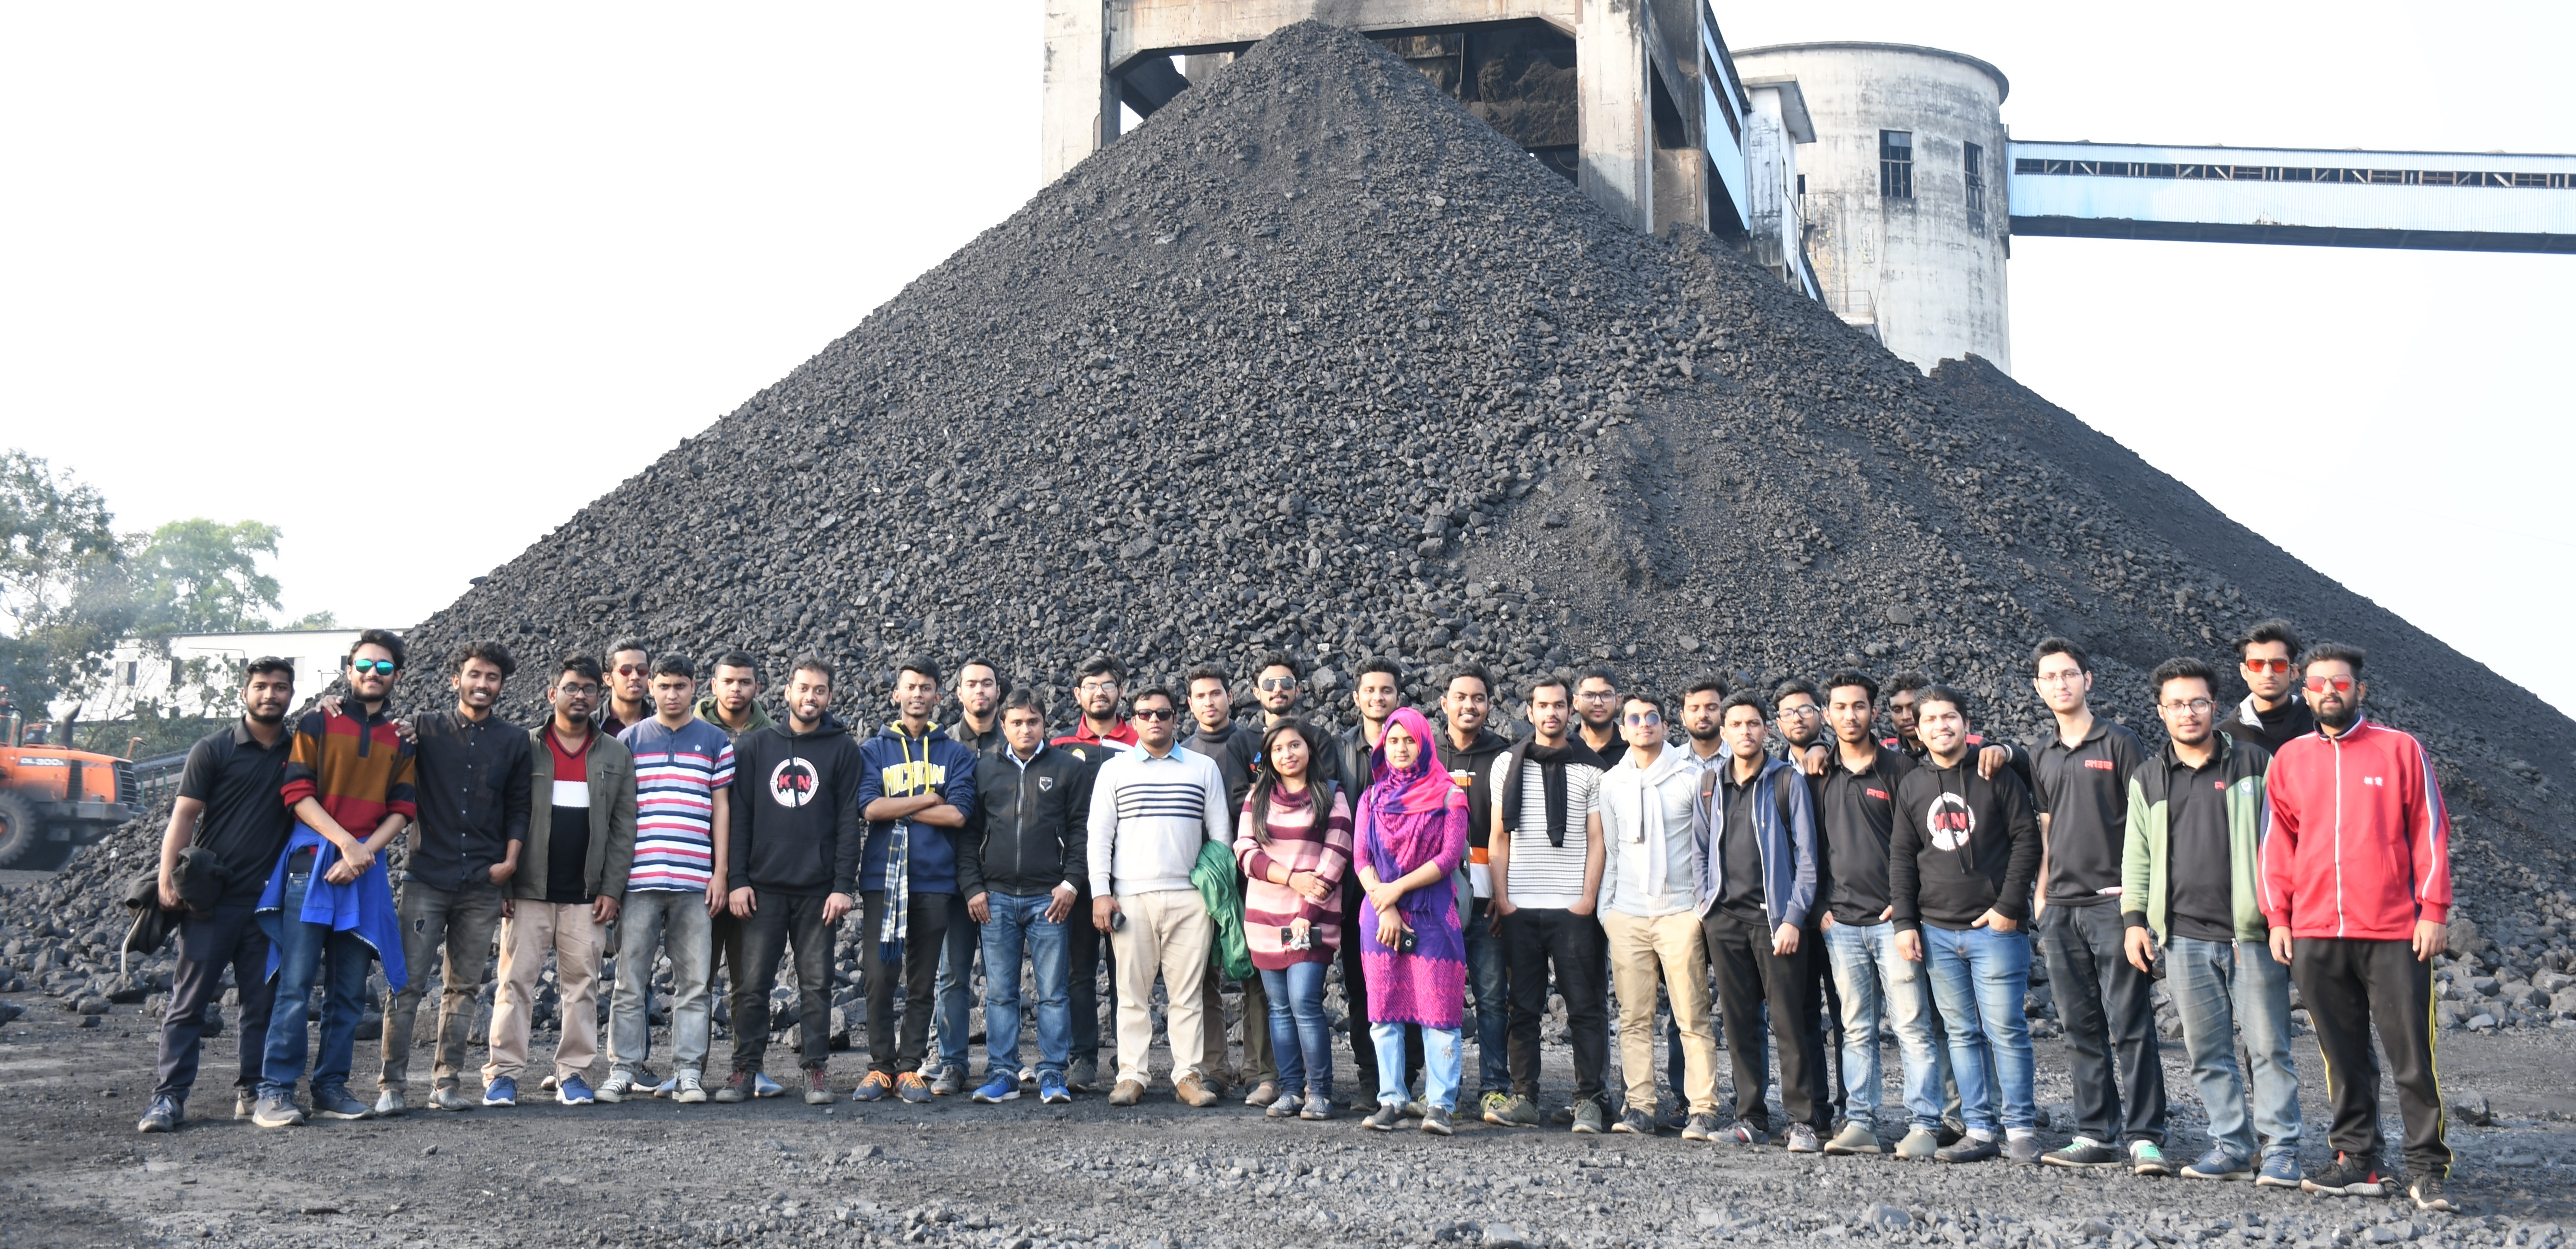
\includegraphics[width=0.95\linewidth]{group photo.jpg}}
\caption{Group Photo in Coal Stocking Site}
\end{figure}
\noindent
\\We started our journey on 7 February, 2020 from Sylhet Bus Station. Second day, 8 February, 2020 we visited Maddhapara Granite Mine. At 9 February, 2020 we visited Barapukuria coal mine surface facilities and underground facilities.\\

\noindent
We are very much grateful to our Honorable teachers Mr Mahmudul Hasan, Lecturer, Dept. of PME and Md. Abdullah Al Numanbakth, Lecturer, Dept. of PME. We are filled with deep gratitude for their benevolent guidelines and support to gather vast amount of information in the field and making our journey more enjoyable and successful all along the field trip.
\section{Objectives}
The main purposes of our field trip:
\begin{itemize}
  \item Visualize the mine dewatering and drainage system of mine.
  \item Visiting the subsidence area
  \item Understanding mining method
  \item Visiting surface and underground facilities
\end{itemize}
\section{Study Area}
The Barapukuria coalfield is located in the Parbatipur thana of Dinajpur district, at a distance of about 50 km southeast of Dinajpur town. The nearest railway station is Phulbari is 6 km south of Barapukuria. The study area around Barapukuria includes- Barapukuria bazar, Subsidence area, South-Barapukuria, North-Barapukuria.

\begin{figure}[ht]
\centering
\fbox{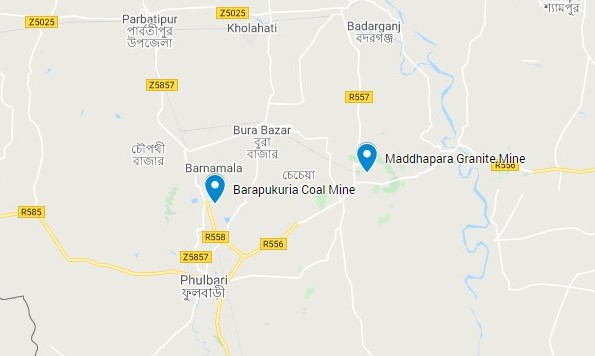
\includegraphics[scale=0.7]{map.jpg}}
\caption{Study Area of Field Trip}
\end{figure}

\noindent
Maddhapara hard rock Mine is located in Maddhapara, Dinajpur, Bangladesh. Maddhapara hard rock Mine is 330 km away from Dhaka, the capital Bangladesh and 14 km away from Phulbari, Dinajpur. The study area around Maddhapara includes- Maddhapara hard rock mine surface visit.\\
the coordinates of both mine are:
\begin{itemize}
\item Maddhapara Granite Mine: 25.5665° N, 89.0647° E
\item Barapukuria Coal Mine: 25.5476° N, 88.9607° E
\end{itemize}

\section{Maddhapara Granite Mine}
\subsection{Geology}
Maddhapara hard rock mine area is located in Rangpur Saddle. The main characteristics of the Saddle are that the sedimentary cover is very thin, and basement lies at shallow depth in this region. It is actually the connecting part of India Shield of Bihar in the west to shilliong shield of Meghaloy if the east. This is why it is called ‘‘the Garo-Rajmahal gap”. Basement found in Maddhapara is probably formed in the Precambrian Era. Maddhapara hard rock mine area is limited to the east by the NW-SE Major fault and to the north by a steep slope of basement. We visited surface facilities of this mine and underground facilities were presented to us by authority.
\subsection{Area, Reserve and Method of the Mine}
\begin{itemize}
\item Mining Method: Room \& Pillar Sublevel Stopping
\item Extent of deposit: $1.2 km^2$
\item present rock reserve: 170 million MT
\item Stope Dimension: $230m\times20m\times60m$
\item Annual Production: 1.65 million MT
\end{itemize}
\begin{figure}[ht]
\centering
\fbox{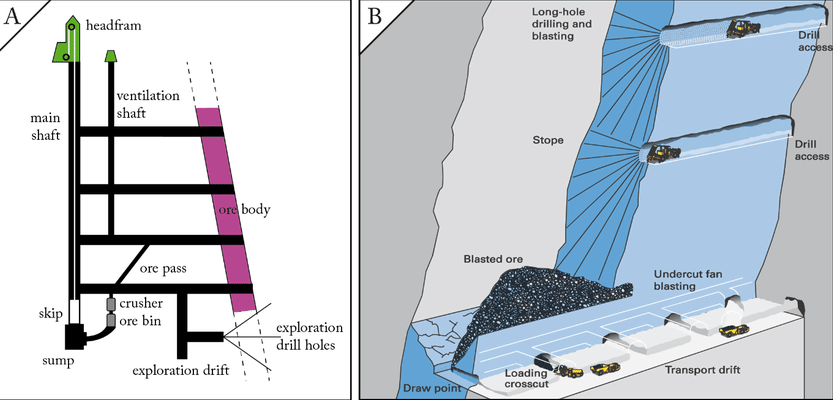
\includegraphics[width=0.95\linewidth]{SublevelStopping.png}}
\caption{Room and Pillar Sublevel Stopping}
\end{figure}

\subsection{Surface Facilities}
\subsubsection{Welfare Building}
This building controlled and supplied the essential mechanical and safety support (wearing cloth, helmet, gum boot, mask) for all Officers, Mine Engineers, and Mine workers during get down and get out from the mine.
\subsubsection{Mine Shaft}
The underground mining operation is operated by two verticals shafts, each of them 5 m in diameter and 240m apart from one another. The shafts are running to the depth of 250 m and 290 m, respectively. The shaft is only one cage and other side is balancing by weight. One shaft is used for hoisting ore material and the other is used for hoisting material, personnel etc. Shaft is also used for ventilation purposes.

\begin{figure}[ht]
\centering
\fbox{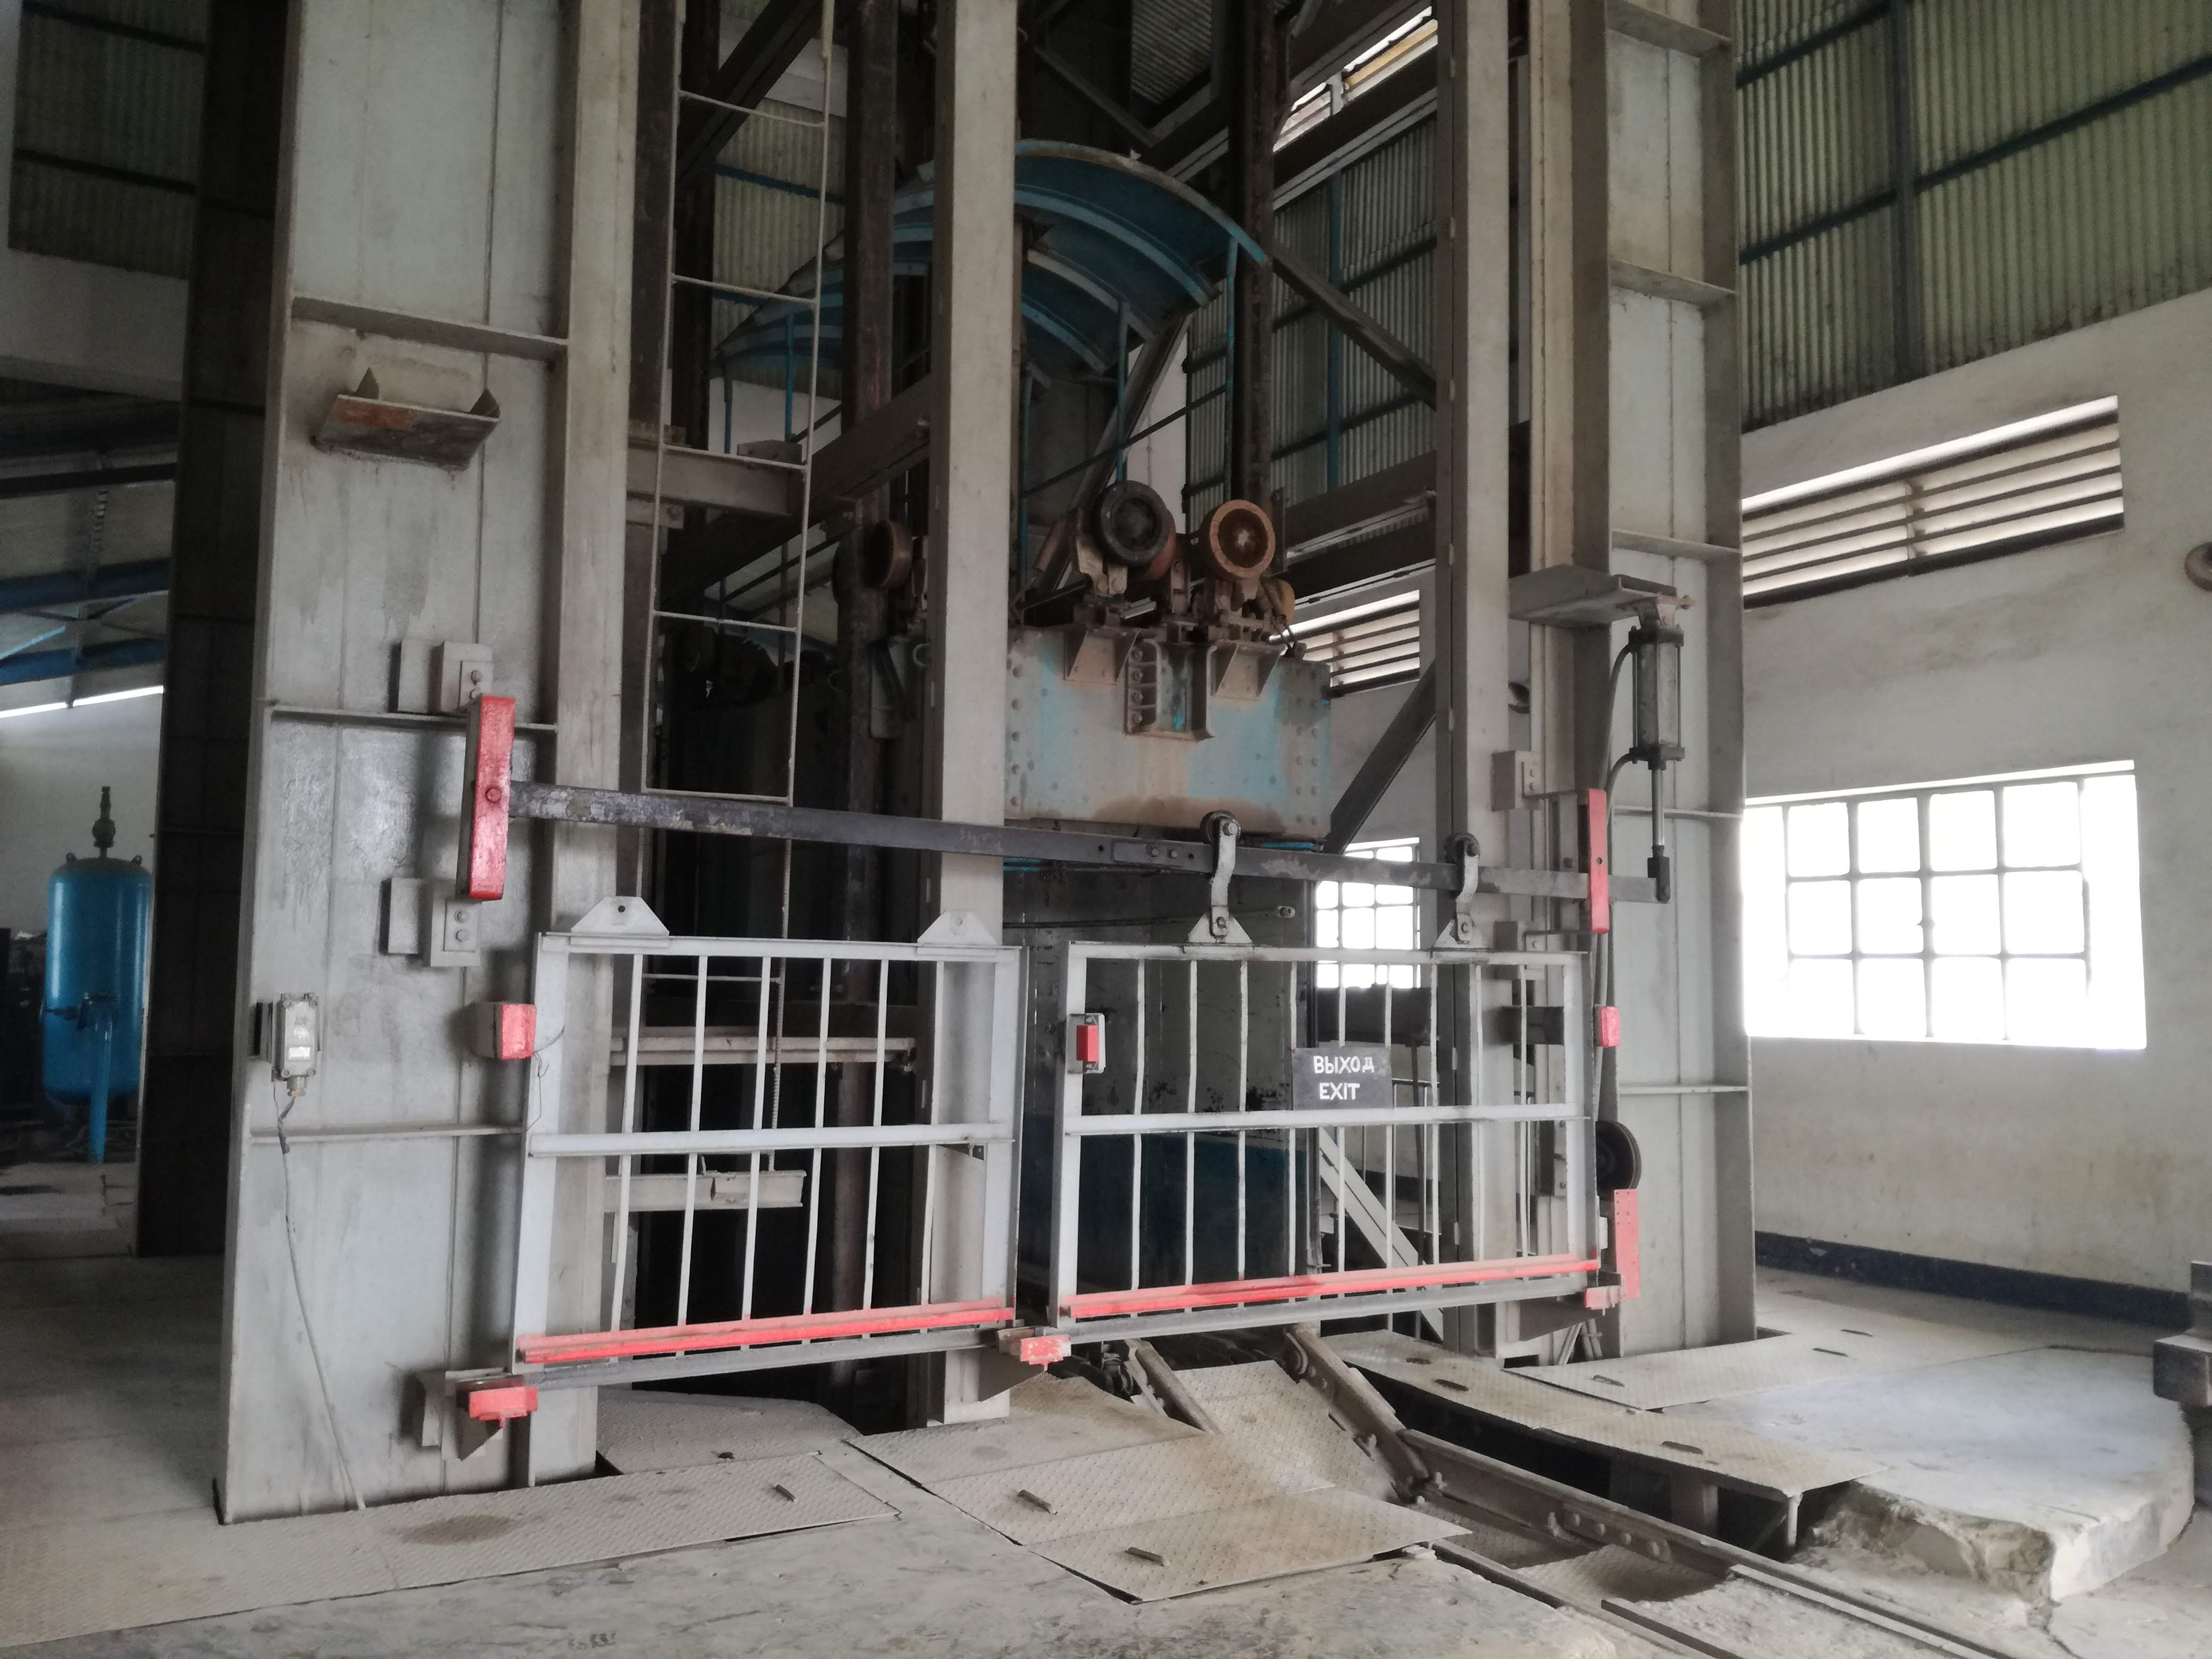
\includegraphics[width=0.9\linewidth]{shaft.jpg}}
\caption{Mine Shaft}
\end{figure}

\subsubsection{Ventilation System}
as shown in figure \ref{ventilation}, Foul air from underground exits through these pipes.

\begin{figure}[t]
\centering
\fbox{\includegraphics[width=0.9\linewidth]{Ventilation.jpg}}
\caption{Ventilation System}
\label{ventilation}
\end{figure}

\subsubsection{Power Station}
There is an electrical substation and generator building. Power Station is used for hoisting purposes, moving conveyor belt, running jaw and cone crusher, ventilation etc. This facility is used in case of power failure. Power Station is shown in figure \ref{powerstation}.

\begin{figure}[ht]
\centering
\fbox{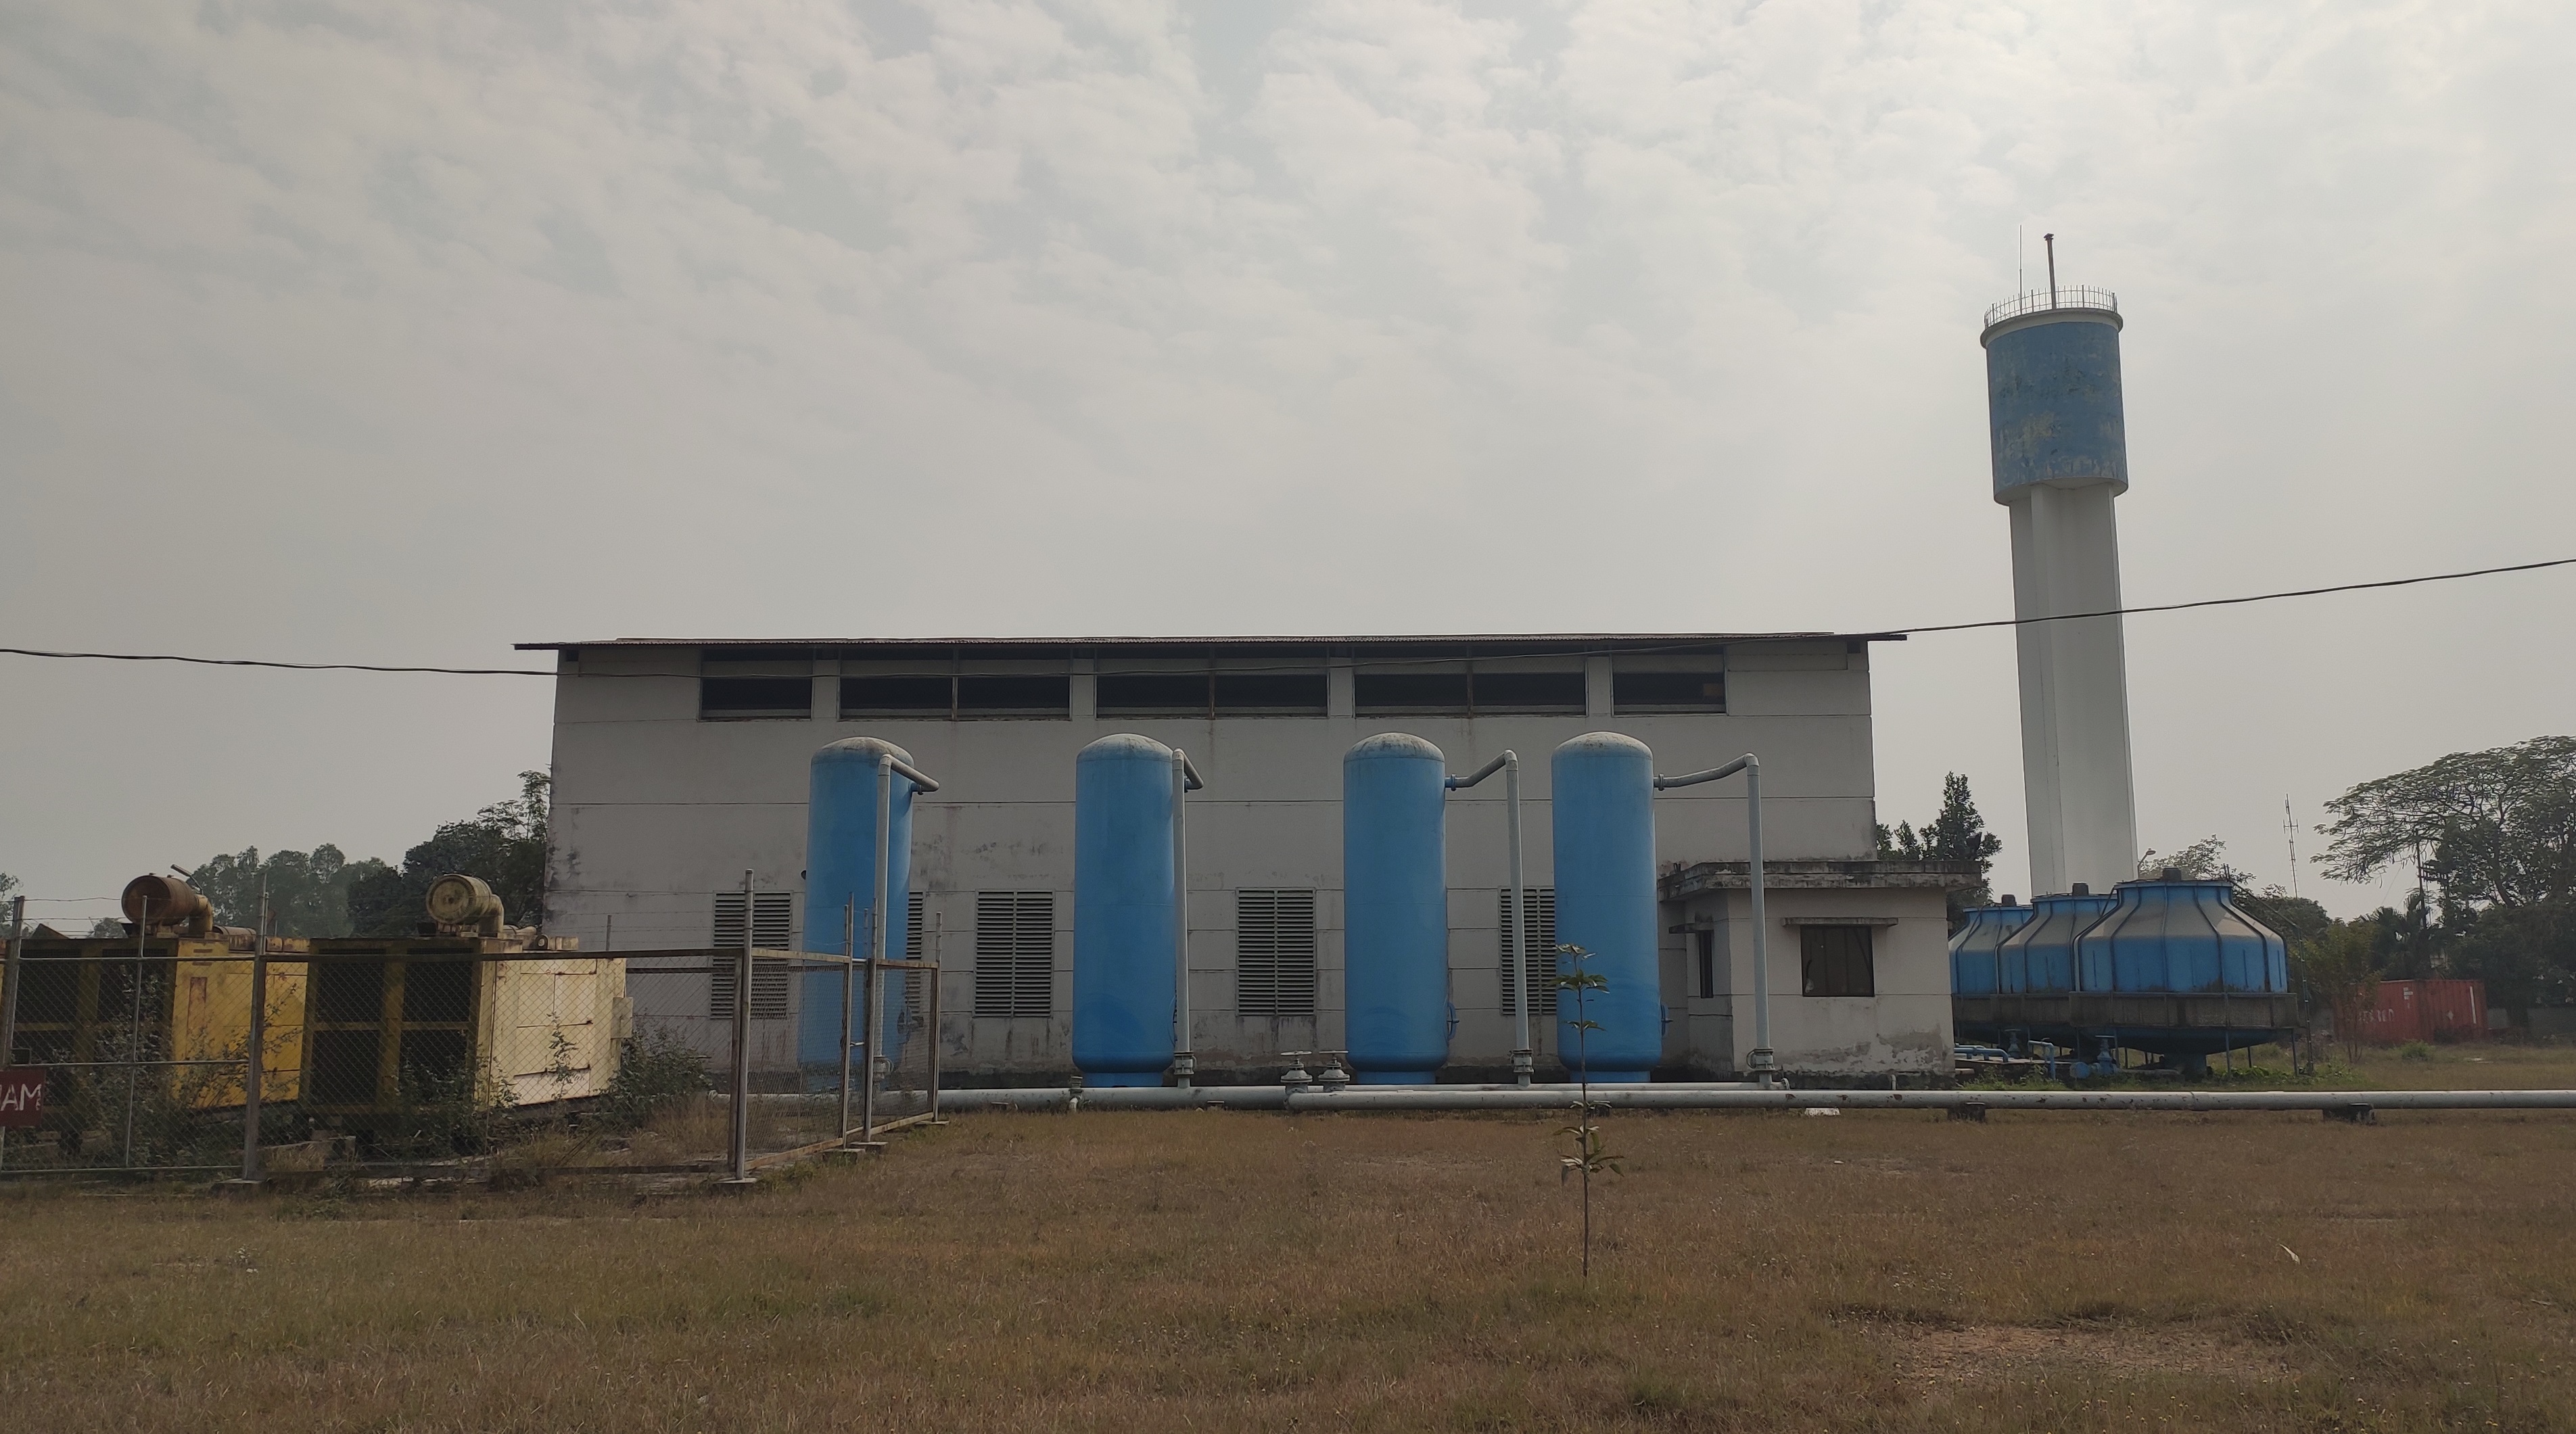
\includegraphics[width=0.9\linewidth]{powerstation.jpg}}
\caption{Electric Sub-Station}
\label{powerstation}
\end{figure}

\subsubsection{Crushing}
Maddhapara Granite Mine produces different size of stone at crushing plant as construction material of which size sand uses are as follows in the table \ref{sizeaftercrushing}. They have three crusher in total, two of them is cone crusher and one is jaw crusher.
\vspace{20pt}
\begin{table}[t]
\caption{size after crushing}
\vspace{5pt}
\centering
\label{sizeaftercrushing}
\begin{tabular}{|c|c|}
\hline
Category                       & Size(in diameter)   \\ \hline
Boulder                        & \textgreater{}250 mm \\ \hline
\multirow{4}{*}{Crushed Stone} & 5-20 mm              \\ \cline{2-2} 
                               & 20-40 mm             \\ \cline{2-2} 
                               & 40-60 mm             \\ \cline{2-2} 
                               & 60-80 mm             \\ \hline
\end{tabular}
\end{table}

\subsection{Underground Facilities}
\subsubsection{Shaft}
The underground mining operation is operated by two verticals shafts, each of them 5 m in diameter and 240 m apart from one another. The shafts are running to the depth of 250 m and 290 m, respectively. The shaft is only one cage and other side is balancing by weight.

\subsubsection{Rail Tracks}
For transporting the granite rail tracks are used. Every bogie can carry 2 tons granite.

\subsubsection{Tunnel}
The tunnel is room and pillar in structure. In the tunnel there is compressed air supply line, signal cables, water supply line, electricity supply line, and locomotive. Three mining development tunnels such Ventilation, production, transportation is excavated at depth level of 194 m, 213 m, 238 m with connection to vertical shafts. As shown in fig \ref{tunnel}, in every tunnel there have rail track to transport rock from blasting area to surge bunker for hoisting out rock to the surface.

\begin{figure}[ht]
\centering
\fbox{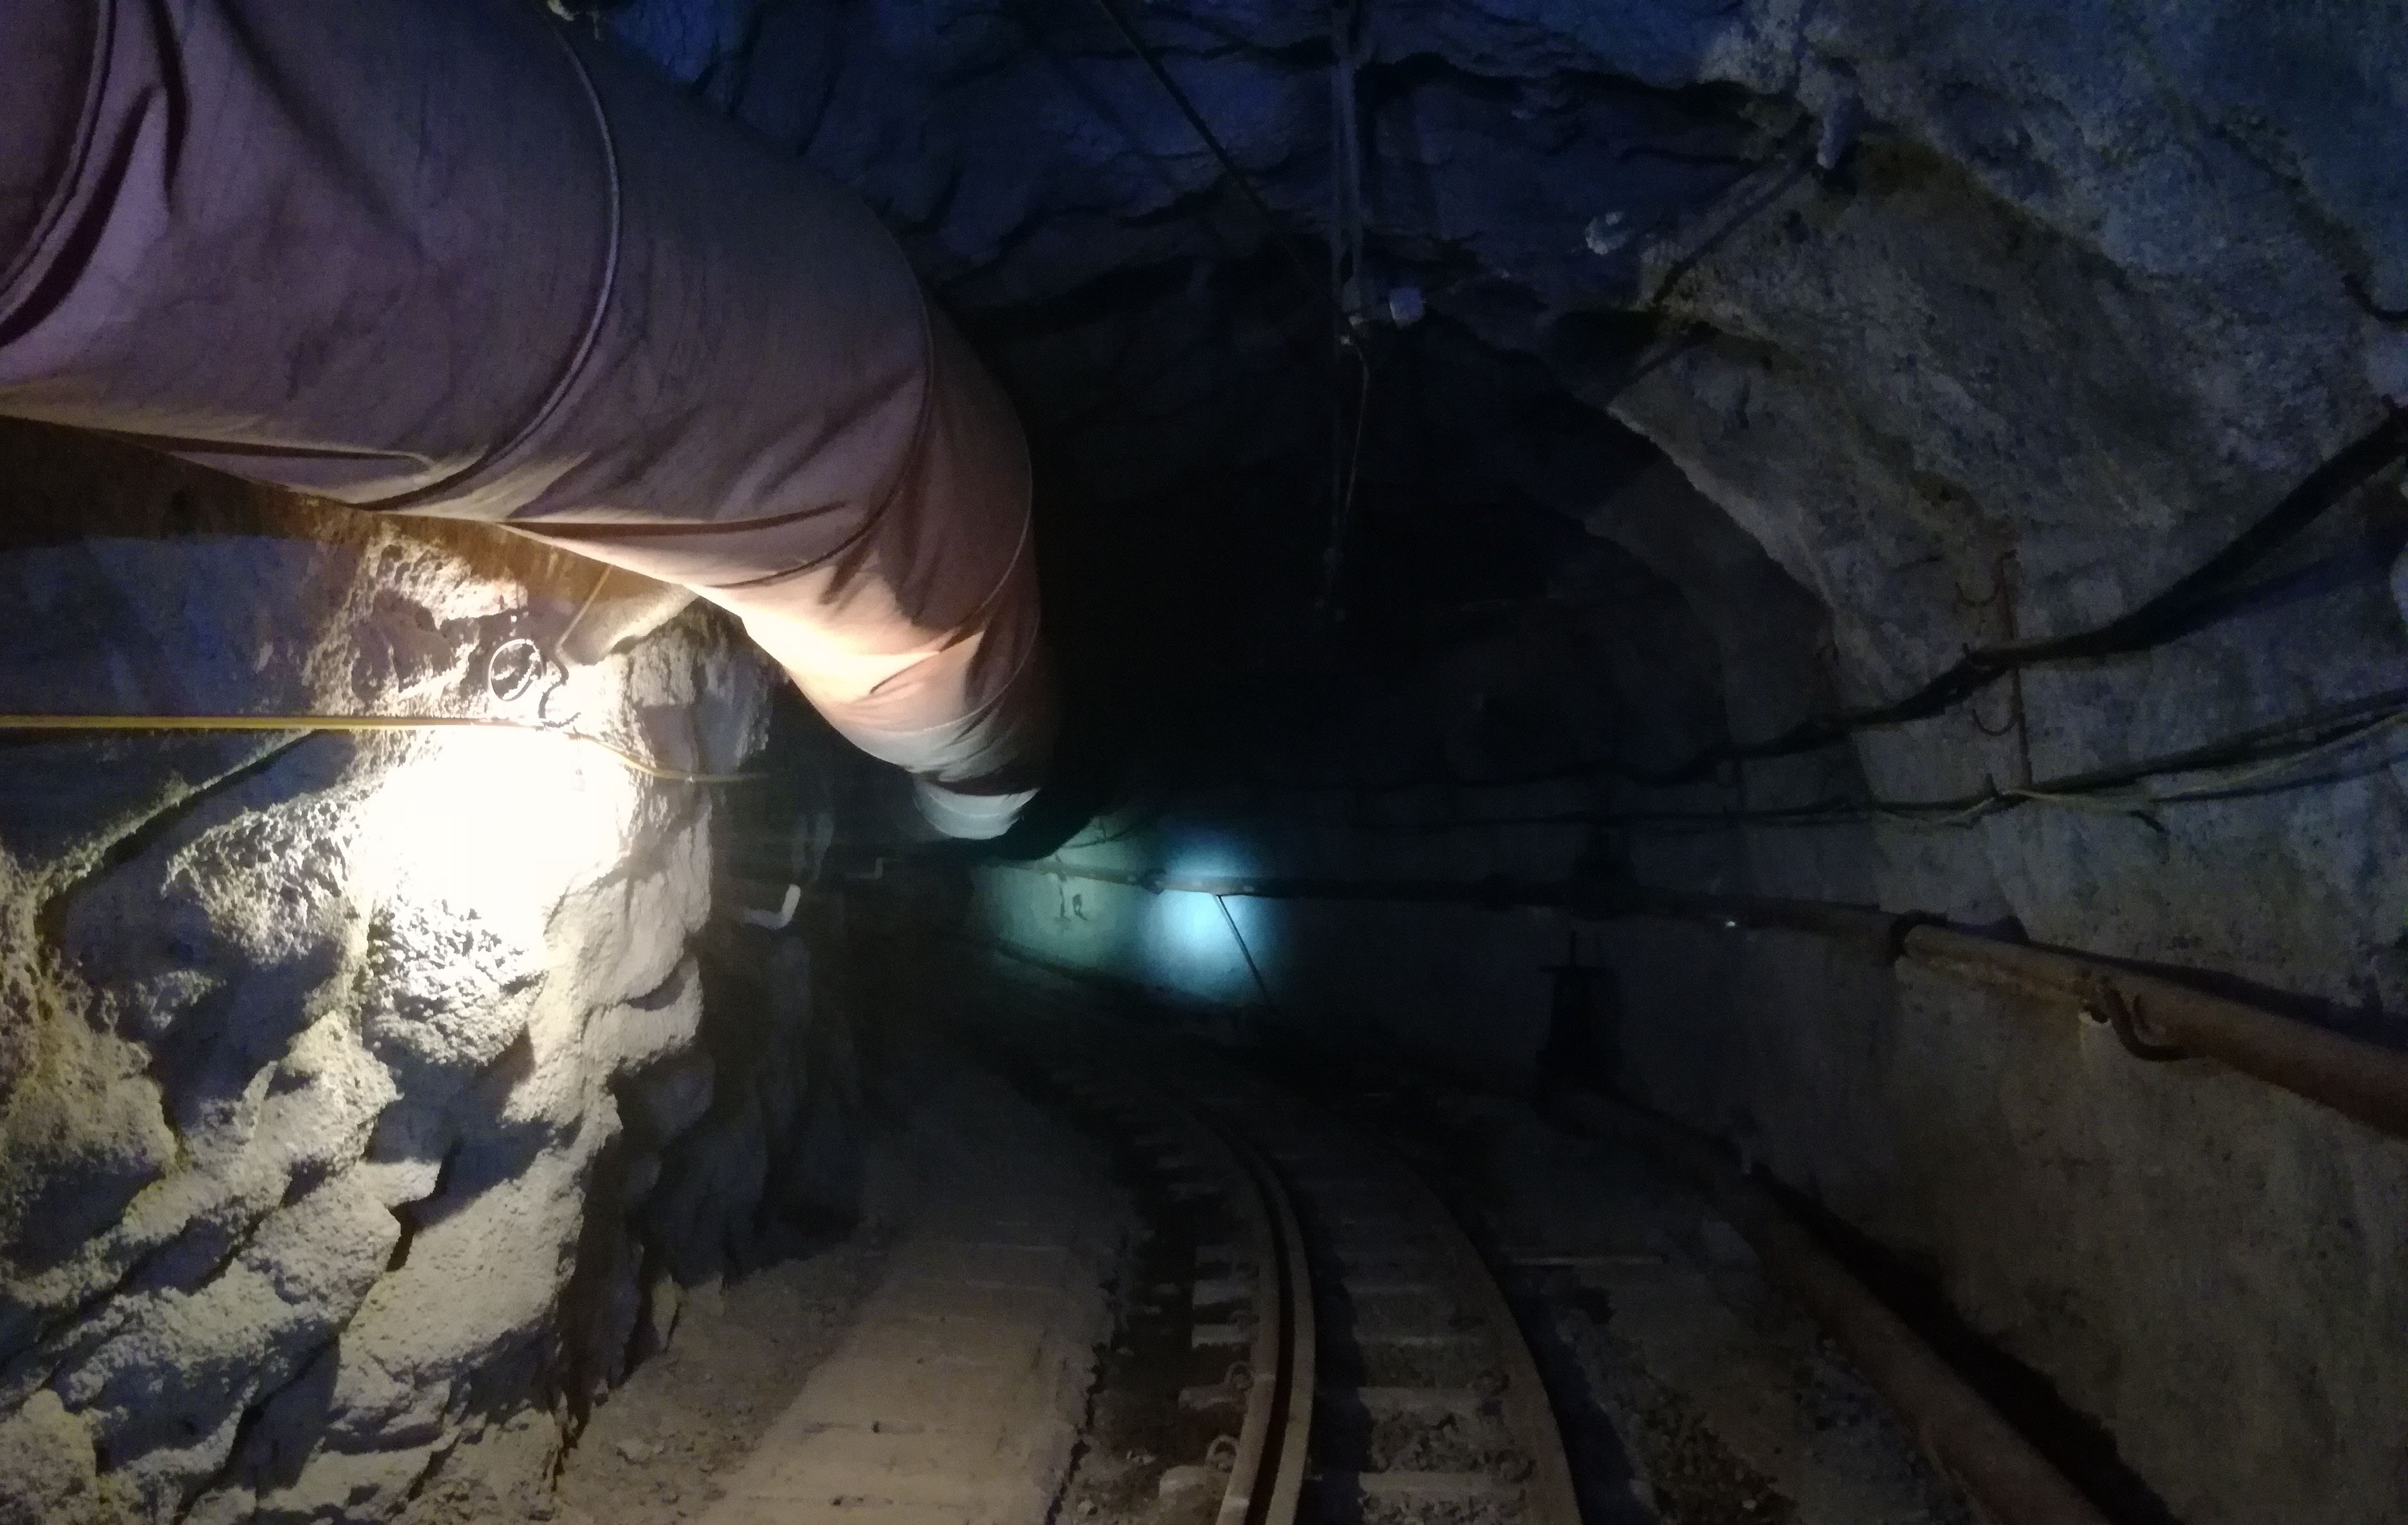
\includegraphics[width =0.9\linewidth]{tunnel.jpg}}
\caption{Tunnel \& Rail Tracks}
\label{tunnel}
\end{figure}

\subsubsection{Locomotives}
They are used to transfer rock. They are electric powered. The locomotives are electrically connected to a high voltage line which power the locomotive.
\begin{figure}[ht]
\centering
\fbox{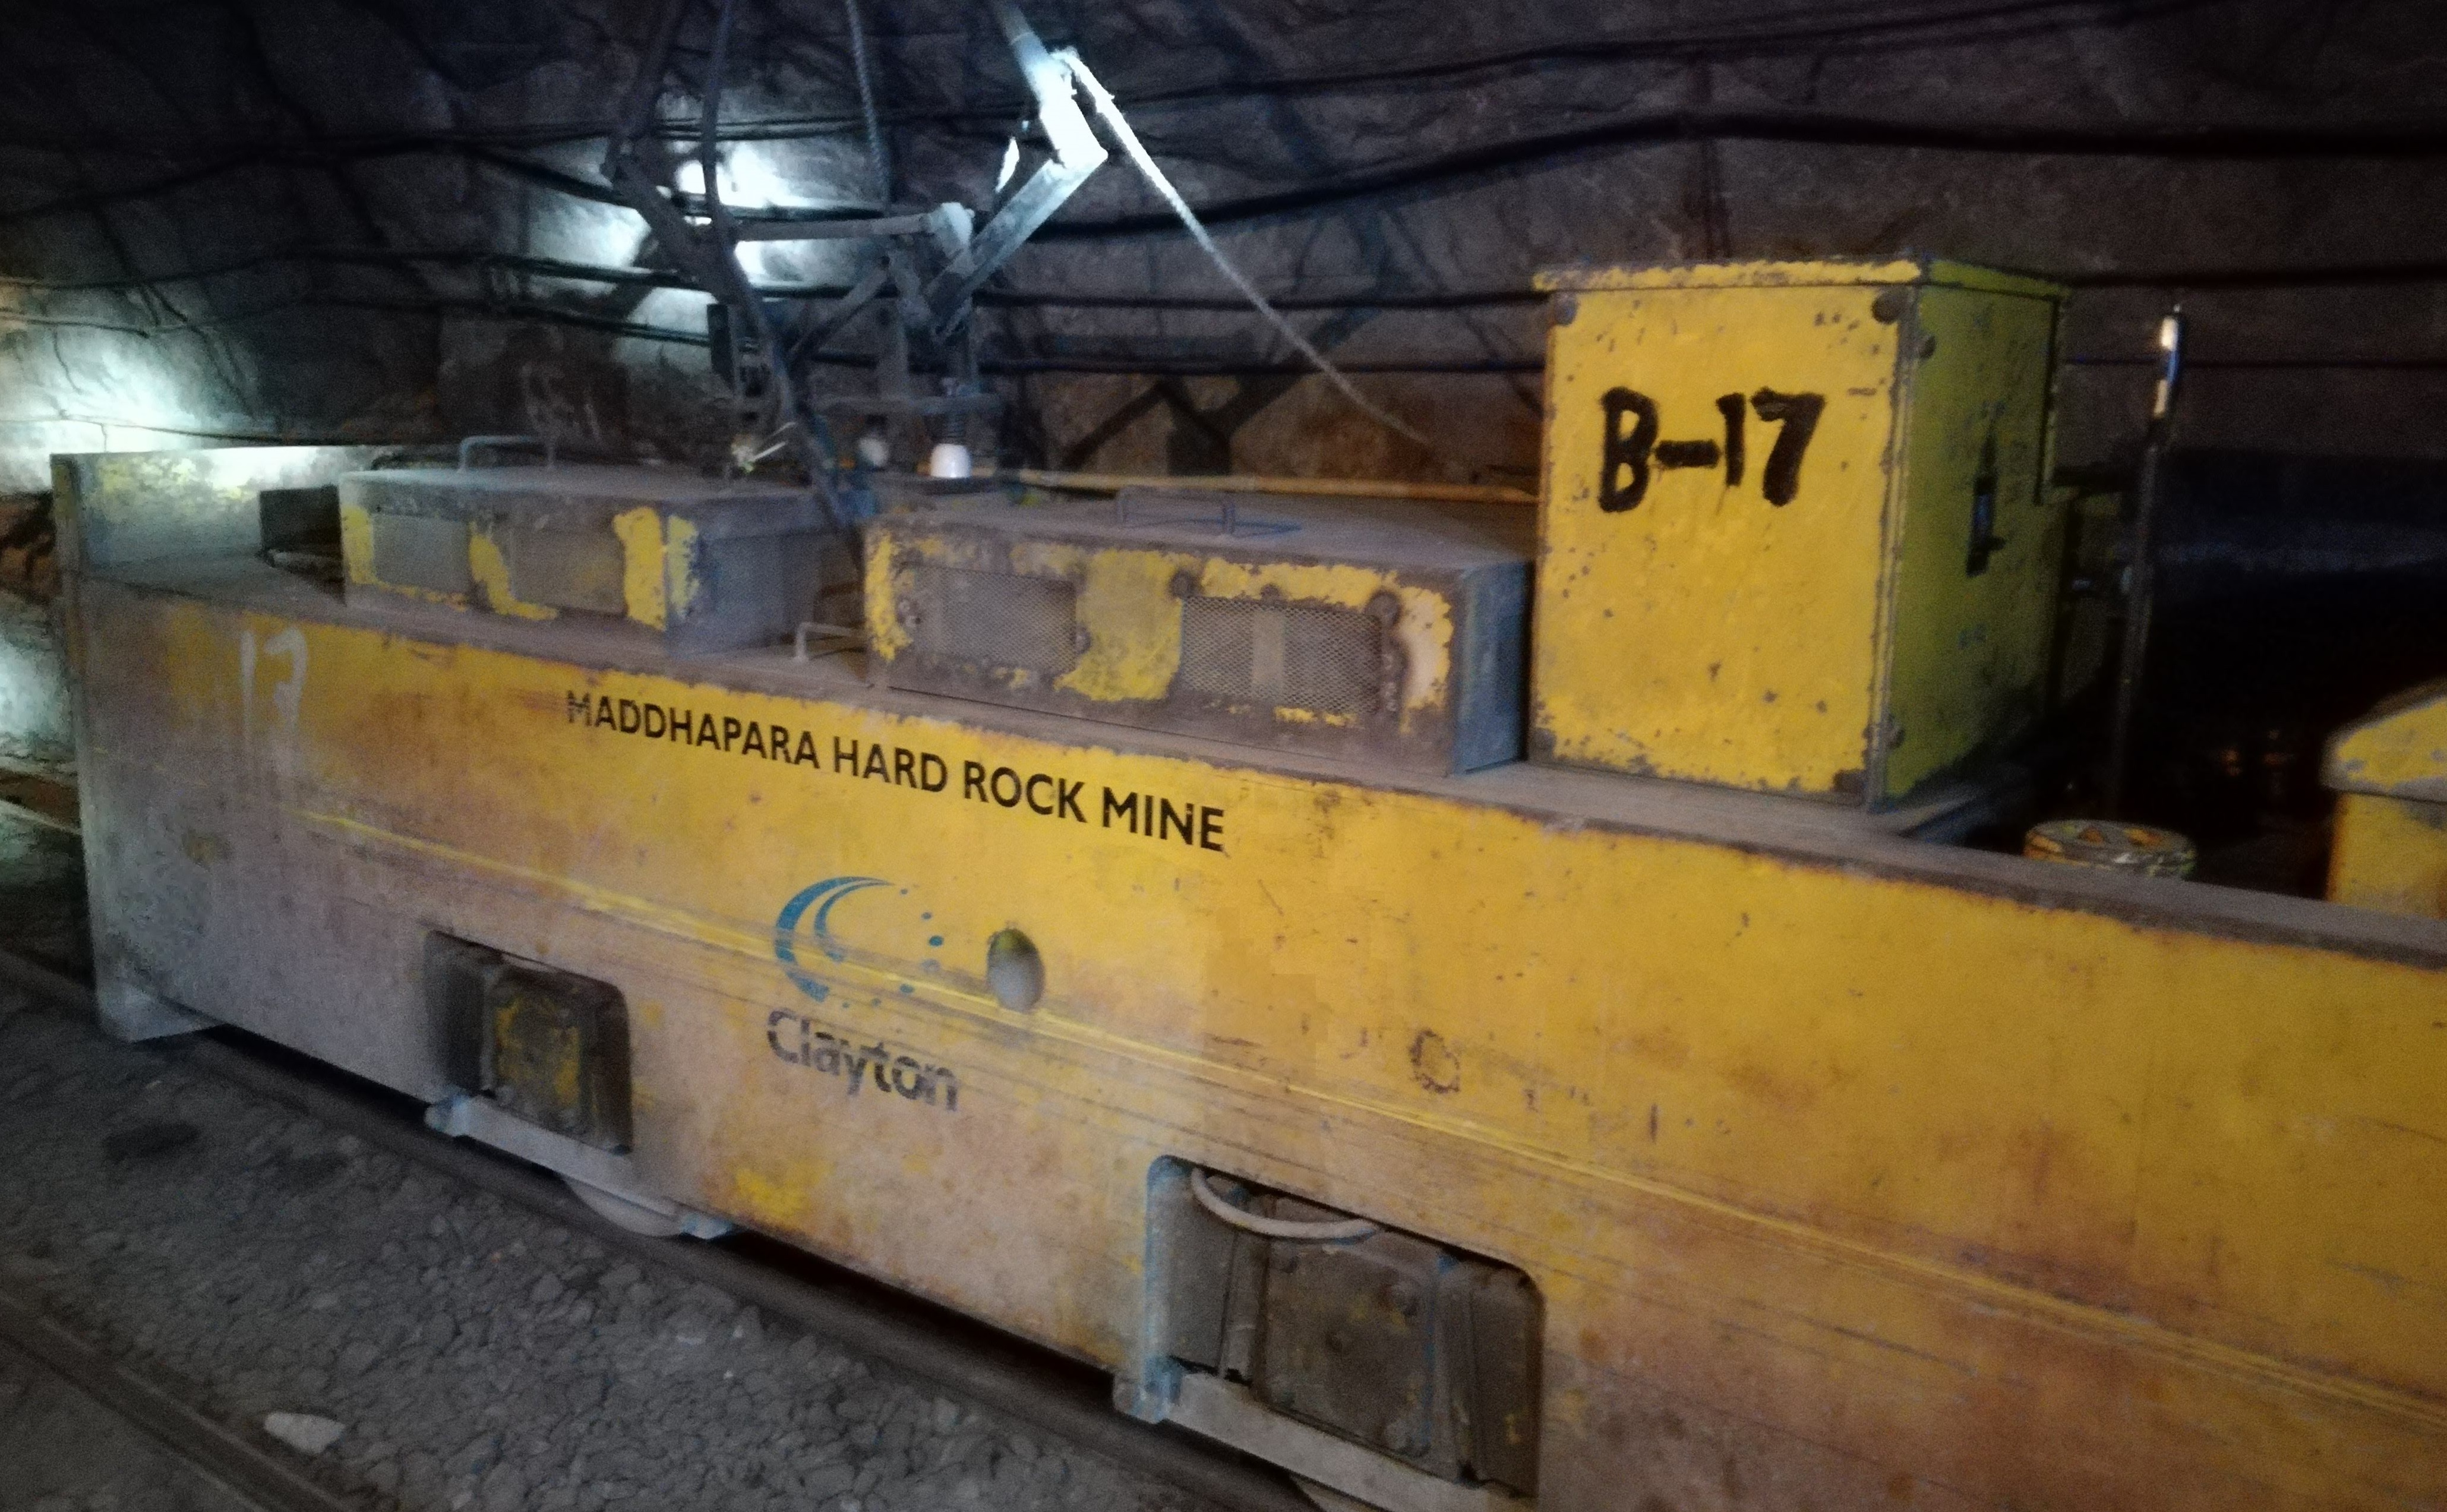
\includegraphics[width =0.9\linewidth]{locomotive.jpg}}
\caption{Locomotive}
\label{locomotive}
\end{figure}

\subsubsection{Pump}
They use 5 six stage centrifugal pump at production level for dewatering purposes and in this level there is also a local power station for locomotive purposes.

\begin{figure}[ht]
\centering
\fbox{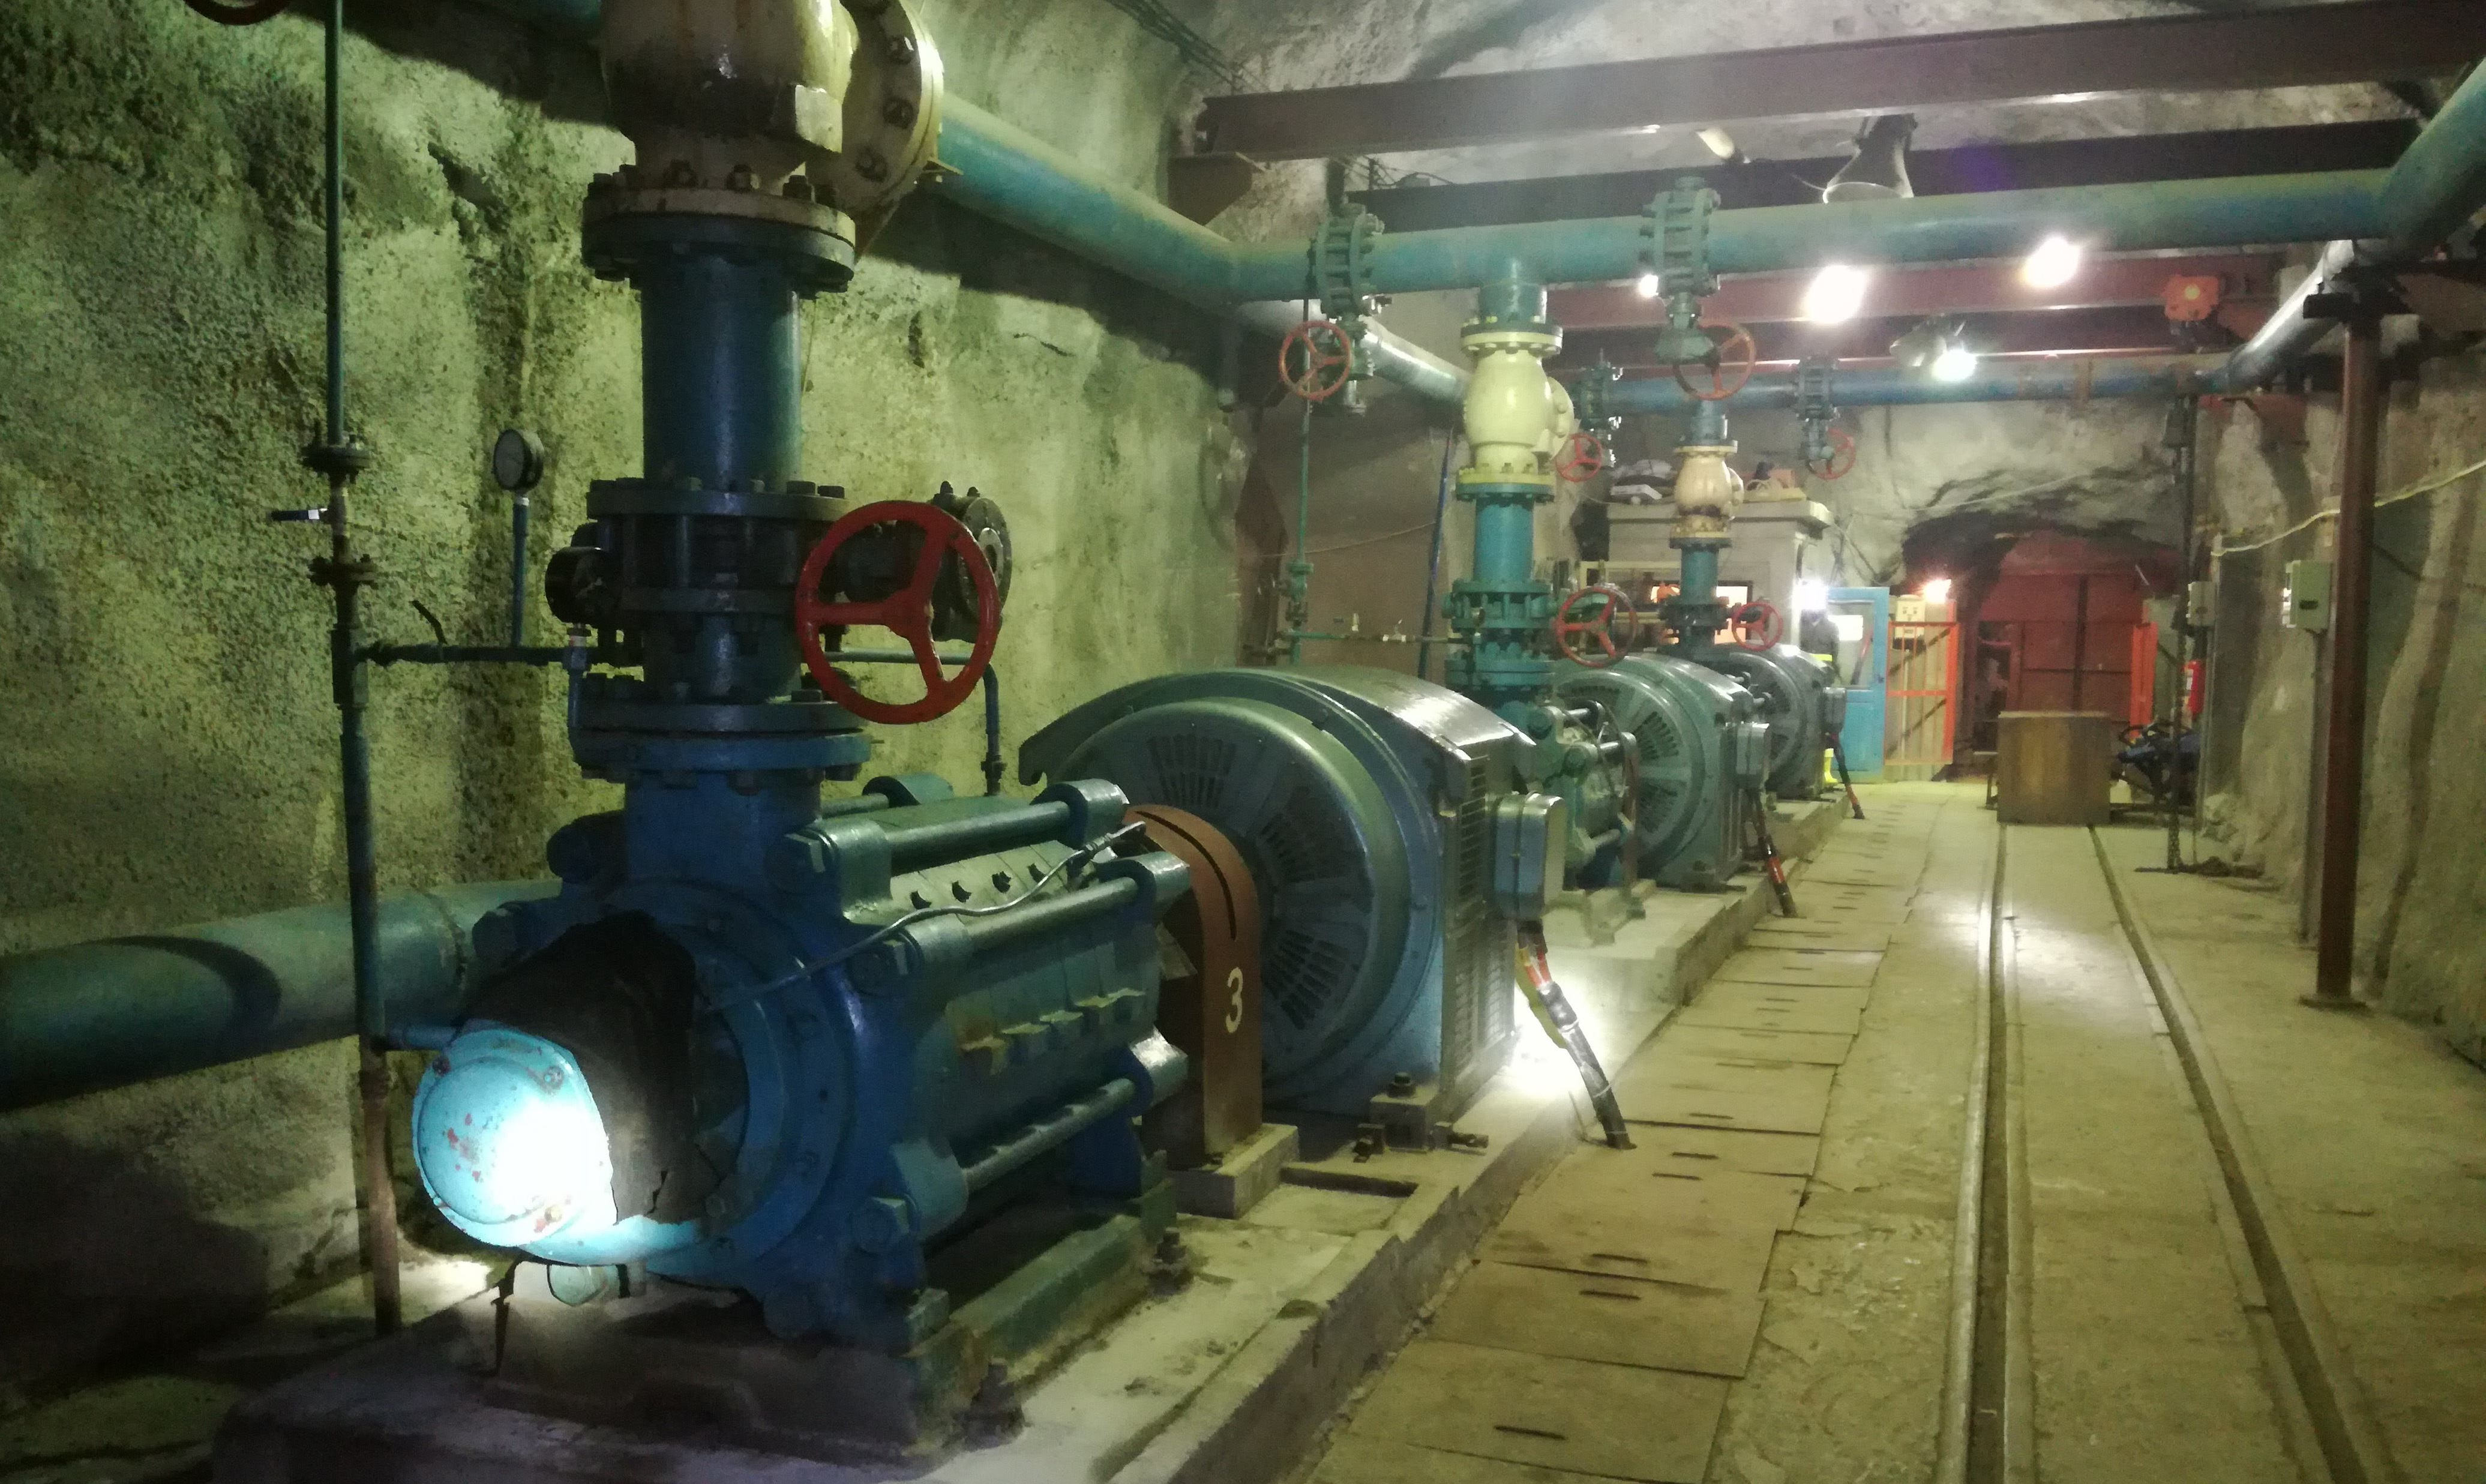
\includegraphics[width =0.9\linewidth]{pump.jpg}}
\caption{Underground Centrifugal Pumps}
\label{pump}
\end{figure}


\subsection{Production Cycle/Process}
In this sub-level stopping system there have three level of horizontal tunneling:
\begin{itemize}
\item Ventilation level
\item Sub level
\item Production level
\end{itemize}
First blasting is occurred in ventilation level then sub-level and after that at production level, the rock is hoisted up from production level via a vertical shaft. As shown is the figure \ref{flowchart}, they sorted the rock into 6 different types according to their grain size.
\begin{figure}[ht]
\centering
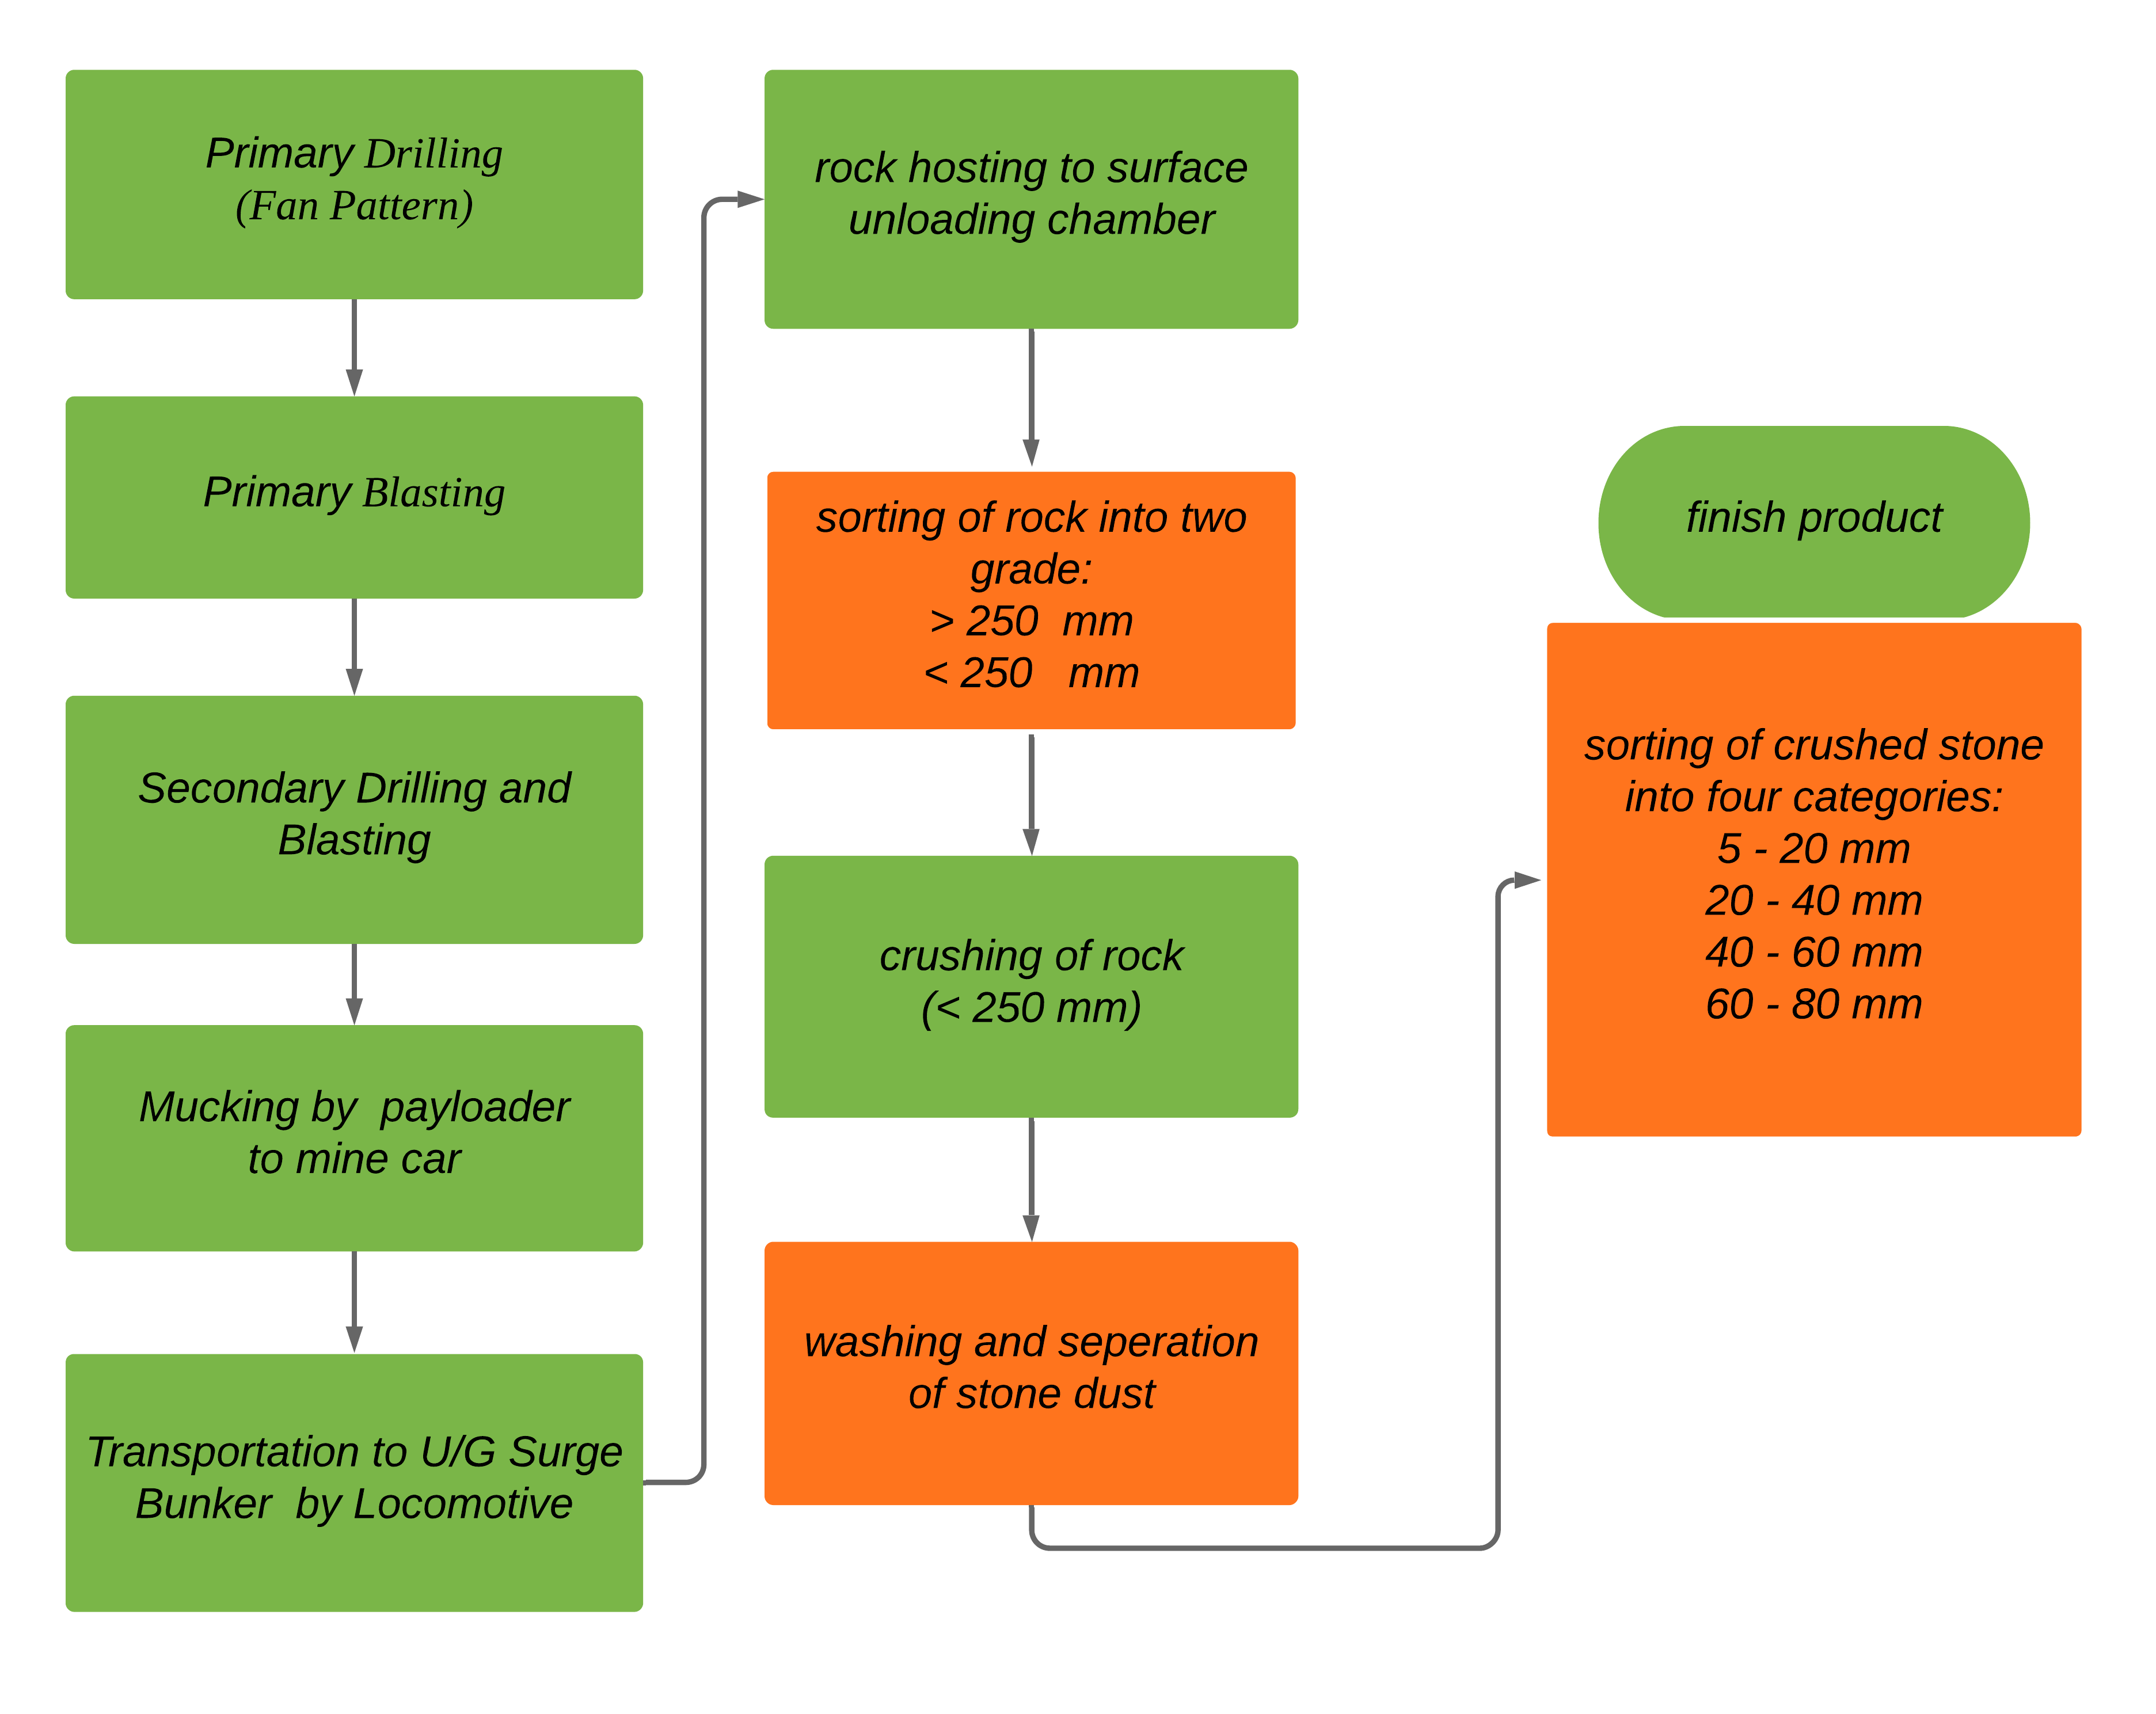
\includegraphics[width=\linewidth, height= 12cm]{flowchart.png}
\caption{Production Cycle of Maddhapara Granite Mine}
\label{flowchart}
\end{figure}
\clearpage

\section{Barapukuria Coal Mine}
\subsection{Geology}
The Barapukuria coal basin is located in the tectonic unit Rangpur saddle of the stable platform in the northwest Bangladesh. The coal bearing sedimentary rocks of the basin lie unconformably on the Precambrian crystalline basement. The basin is elongated in north south direction and has a length of about 4.5 km and a width of about 1.5 km. It is a half graben type asymmetric basin bounded in the east by a major fault known as Eastern Boundary fault. We visited surface facilities, underground facilities, underground dewatering facilities, drainage system of mine water.
\begin{itemize}

\item Area: $6.68 km^2$
\item Depth: $118.57 – 509$ meters
\item Reserve: $390$ million MT
\item Mineable: $64$ million MT

\end{itemize}
\subsection{Mining Method}
Longwall top coal caving (LTCC) is a special type of longwall mining applicable to very thick seams (greater than 4.5 m) where good quality coal is being left because "conventional" longwall equipment has not yet been designed to operate successfully beyond around 5 m mining height. It enables an increased recovery for only an incremental additional cost.
\vspace{10pt}
\begin{figure}[ht]
\centering
\fbox{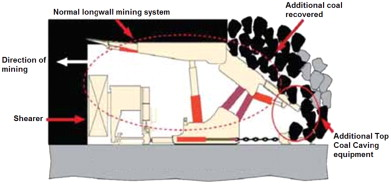
\includegraphics[width=0.9\linewidth]{ltcc.jpg}}
\caption{Longwall Top Coal Caving}
\label{ltcc}
\end{figure}
\clearpage
\subsection{Surface Facilities}

\subsubsection{Shaft}
A pair of vertical shafts is laid in the central shallower part of the basin, on north-south direction.
\begin{itemize}
\item The main shaft depth is 326 m, used for coal hosting and air return of the whole mine.
\item The auxiliary shaft depth is 320 m, used for supplementary hoisting i.e. rocks, materials, equipments, and men, also uses as a function of fresh air inlet in the mine.
\end{itemize} 
\subsubsection{Substation}
To supply electricity in mine operation, buildings etc. substation is working for 24 hours.
\subsubsection{Workshop}
for maintenance of different machineries, rails etc.
\subsubsection{Mine Water Treatment}
Waste water from coal mining process accumulate in slurry pond for settling down and further chemical treatment. For chemical treatment they use $Al_2(SO_4)_3$.

\begin{figure}[ht]
\centering
\fbox{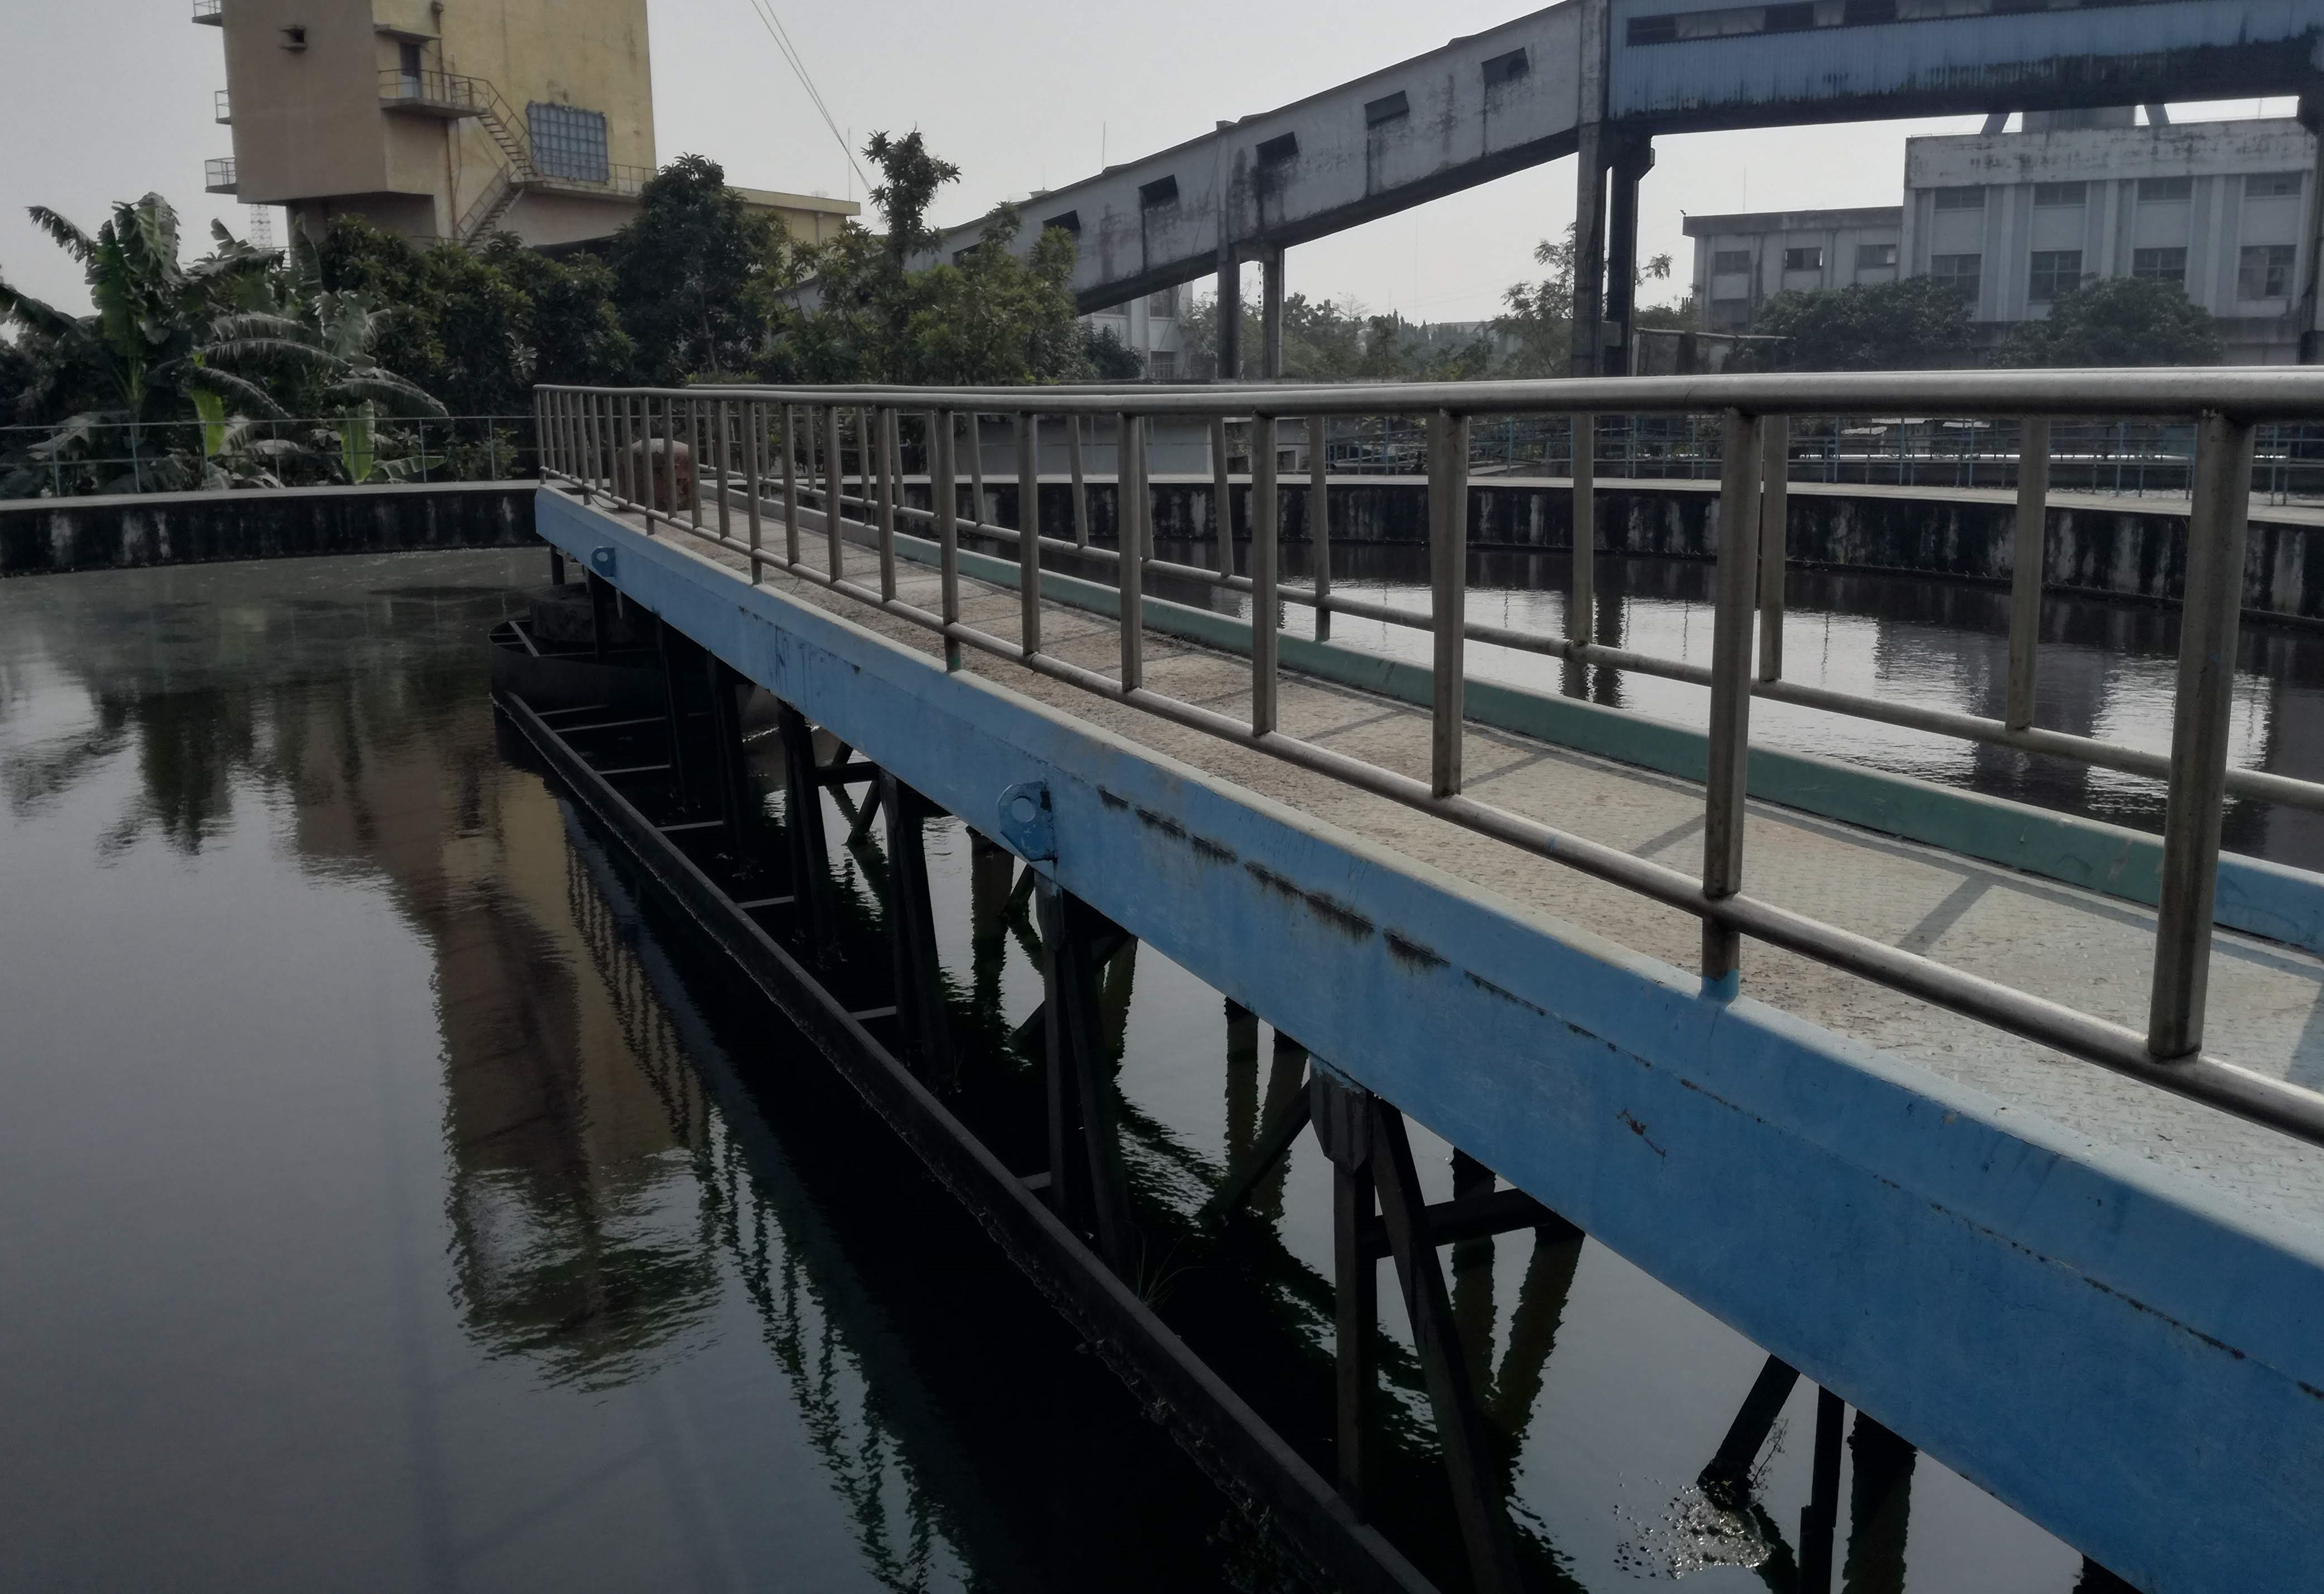
\includegraphics[width=0.9\linewidth]{watertreatment.jpg}}
\caption{Water Treatment System}
\label{watertreatment}
\end{figure}
\clearpage

\subsection{Underground Facilities}
\subsubsection{Level-2}
\begin{itemize}

\item 260 m
\item Through shaft

\end{itemize}
\paragraph{Shaft Stoppage}
Shaft operating room
\paragraph{Power Station}
underground power station for supply electricity
\paragraph{Sump}
A sump is a low space that collects often undesirable liquids such as water or chemicals especially one in the floor of a mine.
\paragraph{Man Rider}
An inclined rail track to move into the underground by electric mine car.
\paragraph{DARR}
DARR refers to Dedicated Air Return Road where foul air exits to the central ventilation system.
\paragraph{Shotcrete Machine}
It is used to make shotcrete for increasing stability of cutting phase.
\subsubsection{Level-3}
\begin{itemize}
\item 390 m
\item Through man-rider
\item Temporary Supporting System
\item Hydraulic Roof Support
\item Shearer
\item AFC for LTCC
\end{itemize}

\subsection{U/G Dewatering}
\begin{itemize}
\item The grey and black water in an underground coal mines naturally mixed abrasives such as small broken stones, small coal particles, sulphur, clay etc drain into sump on this working level.
\item All of the water pumped to surface using Rotary Pump.
\end{itemize}

\subsection{Surface Drainage}
\begin{itemize}
\item Treated water that has been described in figure \ref{watertreatment} is used in underground.
\item Very rough water drained to outside. Figure \ref{drainage} depicts the outside rough water.
\end{itemize}

\begin{figure}[ht]
\centering
\fbox{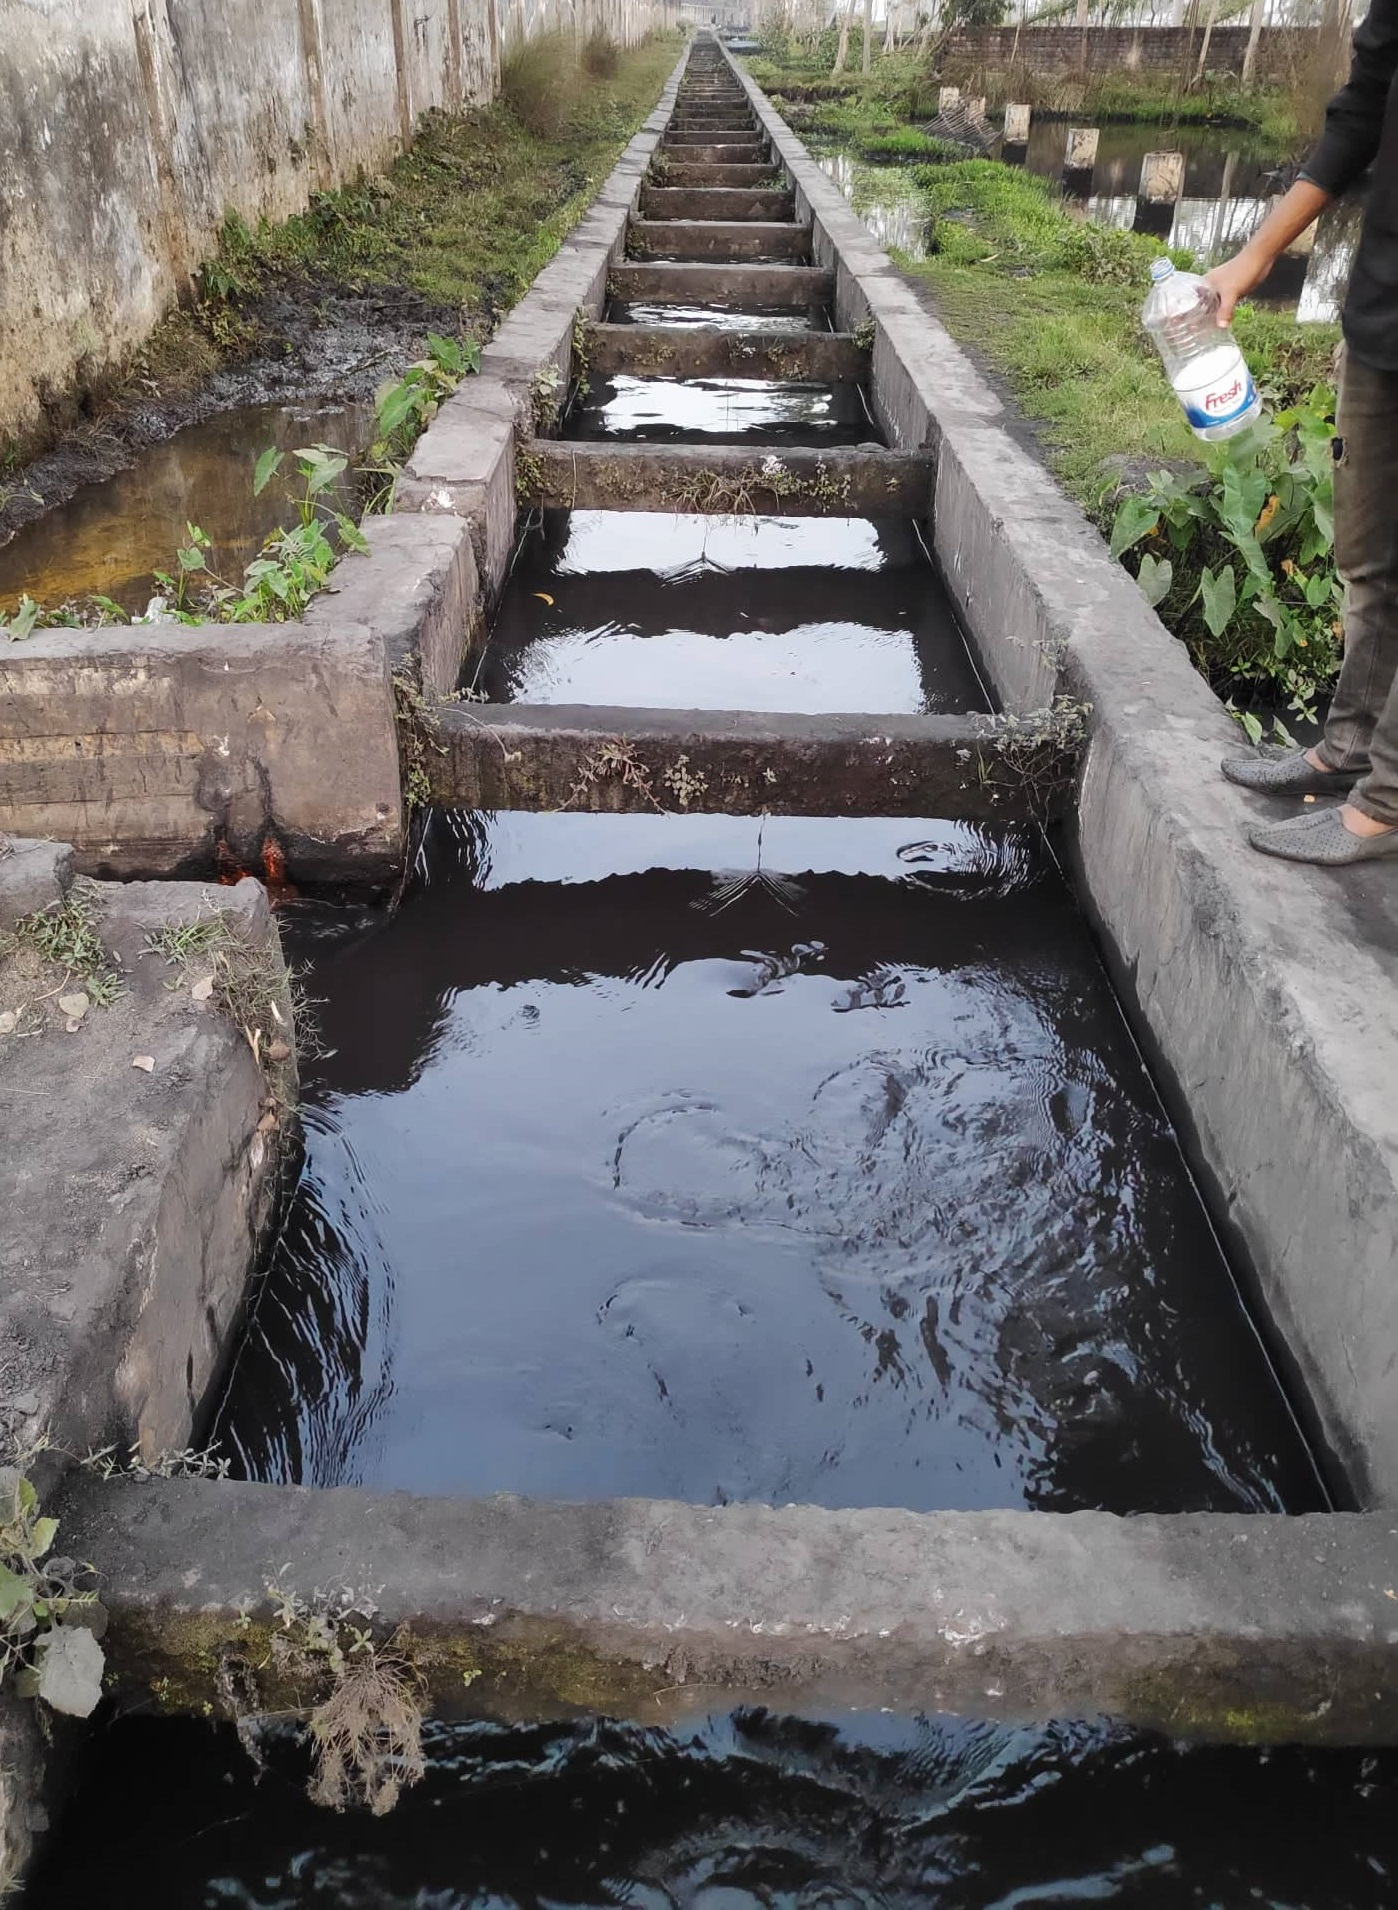
\includegraphics[width=0.9\linewidth]{drainage.jpg}}
\caption{Drainage Water}
\label{drainage}
\end{figure}
\clearpage


\subsection{Subsidence}
Due to extraction of coal continuously surrounding area gradually are going to downward that is termed as trough subsidence. After subsidence, there creates a small depth pit, which eventually became a pond.



\section{Conclusion}
I have achieved a whole new experience in this field tour and learn so many things that i can't put it all in words. I truely believe that this type of tour is necessary for student like us.\\

\noindent
Barapukuria Coal Mine and Maddhpara Granite Mine made a great impact on our economy and will continually pushing up our economy if we utilize this resources properly without any adverse environmental effect.\\
From my observation i think the water management system in both mines especially  in Barapukuria Coal Mine is not as advanced as it should be, and this might impact the nearby soil/water resources and hence degrading our environment. So for this i think proper management of drainage water is necessary.



\vspace{50pt}
\begin{center}
\large{--------- The End ---------}
\end{center}









\end{document}